\documentclass{article}
% \usepackage[a4,  margin=4 cm]{geometry}


% \usepackage{natbib}

\usepackage[utf8]{inputenc}
\usepackage[
backend=biber,
style=alphabetic,
sorting=ynt
]{biblatex}
\usepackage{comment}
\usepackage{csquotes}


%%proof at end


\usepackage[ruled,vlined]{algorithm2e}
\addbibresource{citations.bib}
\usepackage[english]{babel}
\usepackage{url}
\usepackage{mathtools}
\usepackage{enumitem}
\usepackage{dsfont}
\usepackage{bbm}
\usepackage{float}
\usepackage{stmaryrd}
\usepackage[utf8]{inputenc}
\usepackage[T1]{fontenc}
\usepackage{placeins}
\usepackage{amsmath, amsfonts, amssymb}
\usepackage{graphicx}
\usepackage{caption}
\usepackage[nottoc]{tocbibind}
\usepackage[ruled,vlined]{algorithm2e}
\newcommand\tab[1][0.5cm]{\hspace*{#1}}
\newcommand\reals{\mathbb{R}}
\usepackage{amsthm}
\newcommand\tp{\Tilde{P}}
\newcommand\JP{P^{\alpha,\beta}}

\newcommand\tmu{\Tilde{\mu}}
\DeclareMathOperator{\supp}{supp}

\newtheorem{theorem}{Theorem}
\newtheorem{define}{Definition}
\newcommand\jp{p_t^{\alpha,\beta}}
\newtheorem{lemma}[theorem]{Lemma}
%\newtheorem{assumption}[theorem]{Assumption}
\newtheorem{corolary}[theorem]{Corollary}
%\newtheorem{example}[theorem]{Example}

\newtheorem{remark}[theorem]{Remark}
\usepackage[utf8]{inputenc} % allow utf-8 input
\usepackage[T1]{fontenc}    % use 8-bit T1 fonts
%\usepackage{hyperref}       % hyperlinks
\usepackage{url}            % simple URL typesetting
\usepackage{booktabs}       % professional-quality tables
\usepackage{amsfonts}       % blackboard math symbols
\usepackage{nicefrac}       % compact symbols for 1/2, etc.
\usepackage{microtype}      % microtypography

\usepackage{appendix}


\usepackage{empheq}
\usepackage{xcolor, color, colortbl}
\usepackage{framed}
\usepackage{pifont}
\newcommand{\cmark}{\ding{51}}%
\newcommand{\xmark}{\ding{55}}%
\usepackage{enumitem}
% For figures
\usepackage{graphicx} % more modern
%\usepackage{epsfig} % less modern

% to avoid too much space after the algorithm
% \setlength{\textfloatsep}{10pt}% Remove \textfloatsep

\usepackage{nicefrac}
\usepackage{booktabs}
\usepackage{multirow}
\usepackage{rotating}
\usepackage{nccmath}

\usepackage[tikz]{bclogo}
\usepackage{wasysym}

%\SetAlFnt{\normalsize}

\definecolor{mydarkblue}{rgb}{0,0.08,0.45}
\usepackage[
    colorlinks=true,
    linkcolor=mydarkblue,
    citecolor=mydarkblue,
    filecolor=mydarkblue,
    urlcolor=mydarkblue,
    pdfview=FitH]{hyperref}
% smaller url fonts
\usepackage{url}
\usepackage{relsize}
\usepackage{ICLR/iclr2022_conference}
\renewcommand*{\UrlFont}{\ttfamily\smaller\relax}

\newcommand{\blue}{\color{blue}}
\def\xx{{\boldsymbol x}}
\def\yy{{\boldsymbol y}}
\def\zz{{\boldsymbol z}}
\def\qq{{\boldsymbol q}}
\def\dd{{\boldsymbol d}}
\def\XX{{\boldsymbol X}}
\def\YY{{\boldsymbol Y}}
\def\ZZ{{\boldsymbol Z}}
\def\aa{{\boldsymbol a}}
\def\bb{{\boldsymbol b}}
\def\rr{{\boldsymbol r}}
\def\cc{{\boldsymbol c}}
\def\qq{{\boldsymbol q}}
\def\WW{{\boldsymbol W}}
\def\KK{{\boldsymbol K}}
\def\II{{\boldsymbol I}}
\def\yy{{\boldsymbol y}}
\def\vv{{\boldsymbol v}}
\def\uu{{\boldsymbol u}}
\def\ww{{\boldsymbol w}}
\def\zz{{\boldsymbol z}}
\def\SS{{\boldsymbol S}}
\def\BB{{\boldsymbol B}}
\def\AA{{\boldsymbol A}}
\def\CC{{\boldsymbol C}}
\def\MM{{\boldsymbol M}}
\def\DD{{\boldsymbol D}}
\def\PP{{\boldsymbol P}}
\def\TT{{\boldsymbol T}}
\def\VV{{\boldsymbol V}}
\def\bphi{{\boldsymbol \phi}}
\def\QQ{{\boldsymbol Q}}
\def\UU{{\boldsymbol U}}
\def\HH{{\boldsymbol H}}
\def\balpha{{\boldsymbol \alpha}}
\def\bpsi{{\boldsymbol \psi}}
\def\LLambda{{\boldsymbol \Lambda}}
\def\eeps{{\boldsymbol \varepsilon}}
\def\dif{\mathop{}\!\mathrm{d}}
\def\Proba{\mathbb{P}}
\def\MP{\mu_{\mathrm{MP}}}

\def\RR{{\mathbb R}}
\def\EE{{\mathbb{E}}}
\newcommand{\Econd}{\mathbf{E}}
\renewcommand{\gg}{\boldsymbol{g}}
\renewcommand{\vec}{\mathbf{vec}}
\DeclareMathOperator{\prox}{\mathbf{prox}}
\DeclareMathOperator{\tr}{tr}
\def\defas{\stackrel{\text{def}}{=}}
\DeclareMathOperator*{\dom}{dom}
% \DeclareMathOperator*{\supp}{supp}
\DeclareMathOperator*{\Fix}{Fix}
\DeclareMathOperator*{\Var}{Var}
\DeclareMathOperator*{\Span}{\mathbf{span}}
\DeclareMathOperator*{\Deg}{{deg}}
\DeclareMathOperator*{\Trace}{{tr}}

% \newcommand{\xdownarrow}[1]{%
%   {\left\downarrow\vbox to #1{}\right.\kern-\nulldelimiterspace}
% }


\newcommand*\mybluebox[1]{\colorbox{myblue}{\hspace{1em}#1\hspace{1em}}}

\DeclareMathOperator*{\argmin}{{arg\,min}}
\DeclareMathOperator*{\minimize}{minimize}
\DeclareMathOperator*{\diag}{\mathbf{diag}}

\definecolor{myblue}{HTML}{D2E4FC}
\definecolor{Gray}{gray}{0.92}
    
\newtheorem{definition}{Definition}
\newtheorem{example}{Example}
% \newtheorem{remark}{Remark}
\newtheorem{assumption}{Assumption}
% \newtheorem{lemma}{Lemma}
% \newtheorem{proof}{Proof}
\newtheorem{proposition}{Proposition}
% \newtheorem{theorem}{Theorem}


\usepackage{thmtools}
\usepackage{thm-restate}

\usepackage{wrapfig}

\declaretheorem[name=Theorem,numberwithin=section]{thm}
\declaretheorem[name=Proposition,numberwithin=section]{prop}

\DeclareDocumentCommand{\Prto} {o} {
  \IfNoValueTF {#1}
  {\overset{\Pr}{\longrightarrow}}
  { \xrightarrow[ #1 \to \infty]{\Pr }}
}
\usepackage{float}
\usepackage{wrapfig}
%\usepackage[demo]{graphicx}

\title{Only tails matter:
Average-Case Universality and Robustness in the Convex Regime}

\author{Leonardo Cunha
\and Gauthier Gidel \\
\and Fabian Pedregosa \\
\and Courtney Paquette \\
\and Damien Scieur}


\date{August 2021}

\begin{document}
\maketitle
\begin{abstract}
    Recent works have studied the average convergence properties of first-order optimization methods on distributions of quadratic problems. 
    The average-case framework allows a more fine-grained and representative analysis of convergence than the usual worst-case analysis in exchange for a more precise hypothesis over the data generating process, namely the expected spectral distribution (e.s.d) of the random matrix associated to the loss function. 
    In this work, we show that a problem's asymptotic complexity is determined by the concentration of near the edges of the e.s.d. of the problem. We argue this is a more grounded hypothesis, i.e. we can feasibly assume approximate concentrations in practical situations,  and that this is effectively a middle ground between the coarseness of the worst-case analysis and the unrealistic hypothesis of an exact spectrum.
    We introduce the Generalized Chebyshev method, asymptotically optimal under a hypothesis on this concentration, and globally optimal when the spectrum is a Beta distribution .
    We compare its performance to the Nesterov method, and gradient descent, and we show that the asymptotic convergence of Nesterov is close to optimum in practical scenarios.
\end{abstract}
\section{Introduction}
The analysis of the average complexity of algorithms has a long story in computer science. Notably, the quicksort algorithm presents a worst-case complexity of $O(n^2)$, but it's average case complexity is $O(n\log n)$ which makes it  empirically very competitive despite it's worst-case complexity. Average case complexity also drives much of the decisions made in cryptography \citep{bogdanov2006average}.

Despite it's relevance, average case analyses are difficult to extend to other algorithms, mainly because of the intrinsic issue of defining what would be a typical a distribution over the problems. Recently though, \cite{pedregosa2020acceleration}  derived a framework to systemically evaluate the complexity of first-order methods when applied on distributions of quadratic minimization problems. This is done by tying the average of the convergence metrics to the \textit{expected spectral distribution} of the problem, which is a well studied object on random matrix theory.

\cite{paquette2020halting}  extended this work by introducing a new noisy generative model for the problems . They further derived the average complexity of the Nesterov Accelerated Method \cite{nesterov2003introductory} on a particular distribution and showed the strong concentration of the metrics around a limiting value as dimensions go to infinite. 


\cite{scieur2020universal} showed that for a strongly convex problem with eigenvalues supported on a contiguous interval, the optimal average case complexity converges asymptotically to the one given by the Polyak Heavy Ball method in the worst-case.  

In this work, we approach the non-strongly convex case, with a focus on the smooth subcase. In this scenario optimization drastically slows down, as gradient descent presents worst-case convergence in $\Theta(\frac{1}{t})$ and Nesterov is $\Theta(\frac{1}{t^2})$, where $t$ is the number of iterations, which matches a lower bound on worst-case convergence up to a constant factor \citep{nesterov2003introductory}. 


In this paper, we show that the worst-case complexity of optimization methods on convex problem is much more pessimistic that their average-case. That is, there is a gap between the two analyses. This result is in opposition with the strongly convex case, where both the worst case and average case are asymptotically equal.
%In this paper, we show that, differently from the strongly convex case where the worst-case and average case rates are asymptotically the same, in the simply convex scenario, the worst-case is much more pessimistic than the average-case. That is there is an strict gap between the asymptotic rates in both analysis. Especially in high dimensions  the problem has enough degrees of freedom to be highly adversarial. 

%The different sublinear rates of convergence are of great consequence in the context of large scale algorithms. A sublinear improvement in this scenario can translate to many hours of computation, or yet be the difference between a feasible and unfeasible problem.


A drawback on average case analysis is that it relies, \textit{a priori}, on a much stronger hypothesis,  the \textit{expected spectral distribution} as we will see, when compared to the worst-case analysis, that relies only on the values of the edges of this distribution. 

One of our contributions a middle ground between the strength of these two assumptions, allowing for a \emph{robust} analysis of the average case convergence. That is, we compare the algorithm's performance under different notions of uncertainty on the spectrum. This allows us  to choose the best algorithm for a practical problem based in realistic, i.e. imperfect, information.

The paper is organized as follows, in section \ref{section: average case} we present the average case framework first introduced by \cite{pedregosa2020acceleration}. In section 4, we  show that the main aspects of the convergence, which from an optimization point view are the asymptotic rates, are determined by a low dimensional characterization of the distribution. Parametrizing the distributions in terms of the \textbf{concentration} of the eigenvalues around the edges allows us to effectively determine the precise rates for all continuous distributions supported in an interval $]0,L[$, where $L$ is the largest possible eigenvalue. 

Our theoretical rates match numerical simulations and we show that our analysis is representative of the performance of algorithms on real data.

%Finally we'll state our main results : the Nesterov accelerated method asymptotic rate is close to the optimal one for relatively high concentrations of the eigenspectra near $0$, only a $\log$ term under a standard hypothesis. This means the Nesterov method is a very robust choice on practical scenarios.

\begin{figure}[!htb]
\centering
\begin{minipage}{0.45\textwidth} \vspace{0 pt} %
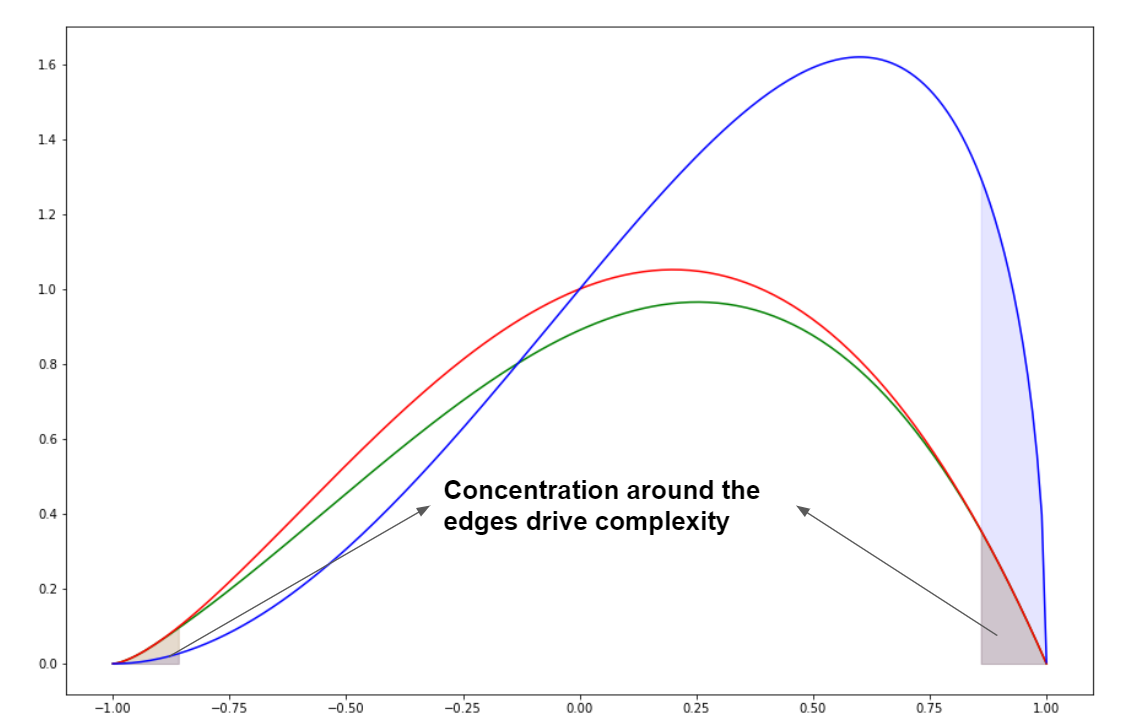
\includegraphics[width = 1.0 \linewidth]{imgs/concentration.PNG}

\begin{small}
\caption{The average case rates for non-strongly problems is determined by the eigenvalue concentration around the edges of the support }
\end{small}
\end{minipage}%
\hfill
\begin{minipage}{0.45 \textwidth} \vspace{0 cm } %
\begin{small}
\captionsetup{type=table} %% tell latex to change to table
    \begin{tabular}{c|c|c}
         Regime&Worst-case& Average-Case  \\
         \hline
         Strongly conv. & $\left(1-\Theta(\frac{1}{\sqrt{\kappa}})\right)^t$ &
         $\left(1-\Theta(\frac{1}{\sqrt{\kappa}})\right)^t$\\ 
         \hline
         Smooth conv. & $\frac{1}{t^2}$ & $\frac{1}{t^{2\xi+4}}$\\
         \hline
          Convex& $\frac{1}{\sqrt{t}}$ & $\frac{1}{t^{\alpha+2}}$
    \end{tabular}
    \vspace{ 0.5 cm}
    %\\ \\ \\ \\ \\ \\ \\
    \caption{Comparison between function value worst-case and average case convergence. $\kappa$ is the condition number in the smooth strongly convex case. In the smooth convex case $\xi$ is the concentration of eigenvalues around $0$ and in the non-smooth case we consider $d\mu\propto \lambda^\alpha e^{-x}$ }\label{table: rates}

\end{small}

\end{minipage}


\end{figure}
\section{Average-Case Analysis} \label{section: average case}


In this section, we recall the average-case analysis framework for random quadratic problems introduced by \cite{pedregosa2020acceleration}.
The main result is Theorem~\ref{thm: metrics}, which relates the expected error  to the \textit{expected spectral distribution} and the \textit{residual polynomial}. The one-to-one correspondence between the residual polynomials and first-order methods applied to quadratics will allow us  to pose the problem of finding an optimal method as a best approximation problem in the space of polynomials.


We recall the definition of a \textbf{random} quadratic problem:
\begin{problem}
Let $\HH \in \RR^{d \times d}$ be a random symmetric positive-definite matrix independent to $\xx^\star \in \RR^d$, a random vector that is the solution to the problem. We define the random quadratic minimization problem as:
\begin{empheq}[box=\mybluebox]{equation*}\tag{OPT}\label{eq:quad_optim}
  \vphantom{\sum_0^i}\min_{\xx \in \RR^d} \Big\{ f(\xx) \defas\!\mfrac{1}{2}(\xx\!-\!\xx^\star)^\top\!\HH(\xx\!-\!\xx^\star) \Big\}\,.
\end{empheq}
We are interested on minimizing the expected errors $\EE \|f(\xx_t) - f(\xx^\star)\|$, the expected function-value gap, and $\EE ||\nabla f(\xx_t)||^2$, the expected gradient norm, where $\xx_t$ is the $t$-th update of a first-order method starting from $\xx_0$ and $\EE$ is the expectation over the random variables $\HH, \xx_0$ and $\xx^\star$.
\end{problem}

The expectation we consider   is over the problem and not over any randomness of the algorithm.%, as would be common in the stochastic literature. In this paper we will only consider deterministic algorithms.


In this paper, we consider the class of \emph{first-order methods} to minimize \ref{eq:quad_optim}. Methods in this class construct the iterates $\xx_t$ as:
\begin{equation} \label{eq:first_order_methods}
    \xx_{t} \in \xx_0 + \Span\{ \nabla f(\xx_0), \ldots, \nabla f(\xx_{t-1})  \}\, .
\end{equation}
That is, $\xx_t$ belongs to the span of previous gradients. This class of algorithms includes for instance gradient descent and momentum, but not quasi-Newton methods, since the preconditioner could allow the iterates to go outside of the span. Furthermore, we will only consider \emph{oblivious} methods, that is, methods in which the coefficients of the update are known in advance and do not depend on previous updates. This leaves out some methods such as conjugate gradient or methods with line-search.


\paragraph{From First-Order Method to Polynomials.}
There is an intimate link between first-order methods and polynomials that simplifies the analysis on quadratic objectives. The next proposition shows that, with this link, we can assign to each optimization method a polynomial that determines its convergence.
% The following proposition states this relationship which relates the error at iteration $t$ with the error at initialization and the residual polynomial.
Following \cite{fischer1996polynomial}, we will say a polynomial $P_t$ is \textit{residual} if $P_t(0)=1$.

\begin{restatable}{proposition}{linkalgopolynomial}
    \label{prop:link_algo_polynomial} \citep{hestenes1952methods}
    Let $\xx_t$ be generated by a first-order method. Then there exists a residual polynomial $P_t$ of degree $t$, that verifies
    \begin{equation}\label{eq:polynomial_iterates}
        \vphantom{\sum^n}\xx_{t}-\xx^\star = P_t(\HH)(\xx_0-\xx^\star)~.
    \end{equation}
\end{restatable}

\begin{remark} \label{rmk: momentum based}
If the first-order method is further a \textbf{momentum method}, i.e.
$$
    \xx_{t+1}=\xx_t+m_t(\xx_t-\xx_{t-1})+h_t\nabla f(\xx_t) .
$$
We can determine the polynomials by the recurrence $P_0=1$ and
    \begin{equation*}
        P_{t+1}(\lambda)=(1+m_t)P_t(\lambda)+h_t\lambda P_t(\lambda)-m_tP_{t-1}(\lambda) .
    \end{equation*}
We note that while most popular F.O.M's can be posed as a momentum method, Nesterov's cannot.
\end{remark}






A convenient way to collect statistics on the spectrum of a matrix is through its \emph{empirical spectral distribution}.


\begin{definition}
(\textbf{Expected spectral distribution [e.s.d]}). 
Let $\HH$ be a random matrix with eigenvalues $\{\lambda_1, \ldots, \lambda_d\}$. The \textbf{empirical spectral distribution} of $\HH$, called ${\mu}_{\HH}$, is the probability measure
\begin{equation}\label{eq:wighted_spectral_density}
    \mu_{\HH} \defas \frac{1}{d}{\textstyle{\sum_{i=1}^d}} \delta_{\lambda_i},
\end{equation}
where $\delta_{\lambda_i}$ is the Dirac delta, a distribution equal to zero everywhere except at $\lambda_i$ and whose integral over the entire real line is equal to one.

Since $\HH$ is random, the empirical spectral distribution $\mu_\HH$ is a random measure (a random variable in the space of measures). Its expectation over $\HH$ is called the \textbf{expected spectral distribution} and we denote it
\begin{equation}
\mu \defas \EE_{\HH}[\mu_{\HH}]\,.
\end{equation}
\end{definition}

We can link the e.s.d. of $\HH$ to the convergence of a first-order method on the distribution of $\HH$. In the following we will consider $\xx_0-\xx^\star$ and $\HH$ to be independent, with $\xx_0-\xx^\star$ sampled isotropically. %This isotropic hypothesis is not necessary and we could derive a similar analysis for more general distribution  of $x_0-x^\star$.

\begin{restatable}{thm}{metrics} \label{thm: metrics}
Let $\xx_t$ be generated by a first-order method associated to the polynomial $P_t$, the measure $\mu$ the  e.s.d. of $H$, and $\mathbb{E}[(\xx_0-\xx^\star)(\xx_0-\xx^\star)^T]=R^2\textbf{I}$ for some constant $R$. Then we can write the convergence metrics at time step  $t$ as
\begin{equation}
\begin{split}
\label{eq:error_norm_x}
  \mathbb{E}[\|\xx_t-\xx^\star\|^2] = { R^2} \int {P_t^2(\lambda) d\mu(\lambda)}, \hspace{1 cm}
    &\mathbb{E}[f(\xx_t)-f(\xx^\star)]=R^2\int P_t^2(\lambda)\lambda d\mu(\lambda)\\
    \text{and} \hspace{1 cm} \mathbb{E}[||\nabla f(\xx_t)||^2_2]&=R^2\int P_t^2(\lambda)\lambda^2d\mu(\lambda) .
\end{split}
\end{equation}
\end{restatable}
This shows that the polynomials are a powerful abstraction as they allows us to write all of our convergence metrics in terms of it . For simplicity, we set $R^2 = 1$ and we will refer directly to the polynomials associated to a given method. We will refer to objective $l$ as the metric associated to the added $\lambda^l$ term, i.e. the function-value is objective $l=1$.

This framework is  linked to the field of \textbf{orthogonal polynomials} by the next proposition. We construct an optimal method w.r.t. a given distribution through a family  of orthogonal polynomials associated to it.


\begin{restatable}{prop}{optimality}\citep{pedregosa2020acceleration}
 \label{prop: optimality}
 Let $P_t^\star$ be defined as
 \begin{equation}
     P_t^\star:={\arg \min}_{P_t(0)=1} \int P_t^2(\lambda) \lambda^l d\nu(\lambda).
 \end{equation}
 Then $(P_t^\star)$ is the family of residual orthogonal polynomials w.r.t. to $\lambda^{l+1}d\nu$.
\end{restatable}

This theorem further implies that the optimal first-order method is a momentum method as Favard's theorem \cite{marcellan2001favard} tells us the orthogonal polynomials w.r.t. a given distribution are related through a \textbf{three term recurrence},

\begin{equation}
    P_{t+1}(\lambda)=a_tP_t(\lambda)+b_t\lambda P_t(\lambda)+(1-a_t)P_{t-1}(\lambda).
\end{equation}
Following Remark \ref{rmk: momentum based}, the optimal method is derived from this recurrence as
\begin{equation}
    \xx_{t+1}=\xx_t+(a_t-1)(\xx_t-\xx_{t-1})+b_t\nabla f(\xx_t)\,.
\end{equation}



\section{Generalized Chebyshev and Laguerre methods} \label{section: methods}
Being able to write the rates in terms of the \textit{expected spectral distribution} ties the average case framework to the field of \textit{random matrix theory}. Indeed, because of results from this field, certain e.s.d's are considered more natural than others. Indeed, the following proposition shows that the same distribution arises when we take the gram matrix of random i.i.d. features. We first recall the definition of weak convergence.%We illustrate this through the following example.

\begin{definition}
We say a sequence of measures $(\mu_n)$ converges weakly to a measure $\mu$ if for any bounded and continuous function $f$ we have
\begin{equation}
    \lim_{n\rightarrow\infty}\int f(x)\dif \mu_n(x)=\int f(x) \dif\mu(x)\,.
\end{equation}

\end{definition}

\begin{prop}[Marchenko Pastur Theorem \citep{bai2010spectral}]
Let $\XX_n$ be a $m\times n$ random matrix with $X_{ij}$ i.i.d with variance $\sigma^2$ and $\YY_n=\frac{1}{n}\XX_n\XX_n^T$. Let $\mu_n$ be the expected spectrum of $\YY_n$, then, as $n\rightarrow\infty$and  $\frac{m}{n} \rightarrow r$

\begin{align*}
&\mu_n\xrightarrow{\text{weakly}}{}\max(0,1-\frac{1}{r})\delta_0+\mu_{MP}, \\
&d\mu_{MP}(\lambda)=\frac{1}{2\pi\sigma^2}\frac{\sqrt{(\lambda^+-\lambda)(\lambda-\lambda^-)}}{r\lambda} ,
\end{align*}
with $\lambda^+=\sigma^2(1+\sqrt{r})^2$, $\lambda^-=\max(0,\sigma^2(1-\sqrt{r})^2)$.

\end{prop}
The Marchenko Pastur distribution $\mu_{MP}$ can be considered a natural first model for e.s.d's as it arises universally from i.i.d. noise in the matrix entries. Note there is no specific distribution of $X_{ij}$ considered. 


When $r=1$, i.e. $n=d$, we have $d\mu_{MP}\propto \lambda^{-1/2}\sqrt{\lambda^+-\lambda}$. Though practical e.s.d's do not take the exact shape of the MP distribution, the same concentration near $0$ is often verified.


\cite{pedregosa2020acceleration} first derived the optimal method w.r.t. $\mu_{MP}$, and \cite{paquette2020halting} derived Nesterov's rates under it. As we are concerned with being robust, a natural step is to consider the Beta weights $d\mu(\lambda)\propto\lambda^\xi(L-\lambda)^\tau$, which can be seen as a generalization of the MP distribution.  Nevertheless, we are mainly interested in distributions with similar concentrations near $0$, i.e. $\xi\approx -1/2$, as this approximate concentration is often found in real data.


The optimal method w.r.t. $\mu$ and metric $l$ is associated to a shifted Jacobi polynomial $\tp_t^{\alpha,\beta}$ with $\beta=\xi+l+1, \alpha=\tau$. When $\alpha=\beta=-1/2$, we retrieve the \textit{Chebyshev Method} \citep{hestenes1952methods}. As such, we call methods of this form the \textit{Generalized Chebyshev Method}. 


We  also consider the Laguerre method, which is optimal w.r.t. $d\mu(x)=\frac{x^\alpha e^{-x}}{\Gamma(\alpha+1)}$, taking $\alpha$ as a parameter. This method is proposed to optimize non-smooth functions.\\
Both these methods are generalizations of one that have been proposed in \cite{pedregosa2020acceleration}. We derive the coefficients associated to these methods in appendix \ref{jacobi recurrence}.\\
\begin{remark}
The Generalized Chebyshev also takes the largest eigenvalue $L$ as a parameter, but the rates we will show are robust to an \textit{overestimation} of $L$.
\end{remark}

\section{Robust Average Case Rates} \label{section: robust average}
We will state our assumption over the spectral distributions. It effectively allows us to parametrize all of our distributions of interest in a way that characterizes the asymptotic convergence, diving them into equivalence classes .

\begin{assumption}
We will write $\nu_{\tau,\xi}$ for a continuous distribution supported in $(0,L]$ s.t. $\nu_{\tau,\xi}'(x)>0$ for $x\in [0,L]$, $d\nu_{\tau,\xi}=\Theta( \lambda^\xi)$ near $0$ and $d\nu_{\tau,\xi}=\Theta( (L-\lambda)^\tau)$ near $L$. 
\label{assumption}
\end{assumption}

We argue this is a much milder assumption to be made than the exact spectral distribution and it covers any distribution modeling a smooth convex problem. 


The $\xi$ works as a measure of how close we are to the worst-case scenario, as it approaches $-1$. Samples in finite dimension, of distributions with high values of $\xi$, will work as strongly convex functions in practice.


We show that $\nu_{\tau,\xi}$ indeed behaves like an equivalence class when considering the asymptotics of the convergence of a Jacobi method: only the concentrations near the edge matter. We do this by singling out from each of these classes the beta distributions for which we can compute the rates, then show the rates to be the same inside $\nu_{\tau,\xi}$.


\begin{restatable}{theorem}{robustjacobi}\label{thm: jacobirates}
A Generalized Chebyshev Method with parameters $(\alpha,\beta)$ applied to a problem with e.s.d. as in assumption \ref{assumption} has rates
\begin{align}
\mathbb{E}[f(\xx_t)-f(\xx^\star)]&\sim L\cdot C^{\alpha,\beta}_{1,\nu}
    \left\{\begin{array}{ll}
    t^{-1-2\beta} &\mbox{if } 
		  \alpha<\tau+1/2 \text{ and } \beta <\xi+3/2\\
		  t^{-2(\xi+2)}\log t& \mbox{if } 
		  \alpha=\tau+1/2 \text{ and } \beta =\xi+3/2\\
		  t^{2(\max\{\alpha-\beta-\tau,-\xi-1\}-1)}& \mbox{if } 
		  \alpha>\tau+1/2 \text{ or } \beta >\xi+3/2
	\end{array}\right. ,\\
	\mathbb{E}[||\nabla f(\xx_t)||^2_2]&\sim L^2\cdot C^{\alpha,\beta}_{2,\nu}
        \left\{\begin{array}{ll}
    t^{-1-2\beta} &\mbox{if } 
		  \alpha<\tau+1/2 \text{ and } \beta <\xi+5/2\\
		  t^{-2(\xi+3)}\log t& \mbox{if } 
		  \alpha=\tau+1/2 \text{ and } \beta =\xi+5/2\\
		  t^{2(\max\{\alpha-\beta-\tau,-\xi-2\}-1)}& \mbox{if } 
		  \alpha>\tau+1/2 \text{ or } \beta >\xi+5/2
	\end{array}\right. ,
\end{align}
where $C^{\alpha,\beta}_\nu$ is a distribution dependent constant.
\end{restatable}

Theorem \ref{thm: optimality} shows that a proper choice of $\alpha,\beta$ can indeed make the Jacobi polynomial asymptotically optimal w.r.t. to any $\nu_{\tau,\xi}$. 

\begin{restatable}{theorem}{jacoptimal}\label{thm: optimality}
Let $\nu$ follow Assumption \ref{assumption}.
The optimal asymptotic rate for $\mathbb{E}[f(\xx_t)-f(\xx^\star)]$ is $t^{-2(\xi+2)}$ and is attained by the Chebyshev Method with parameters $(\tau,\xi+2)$. 


The optimal rate for $\mathbb{E}[||\nabla f(\xx_t)||^2_2]$ is $t^{-2(\xi+3)}$ and is attained by the Chebyshev Method with parameters $(\tau,\xi+3)$.
\end{restatable}

\begin{wrapfigure}{r}{0.6\textwidth}
    \centering
    %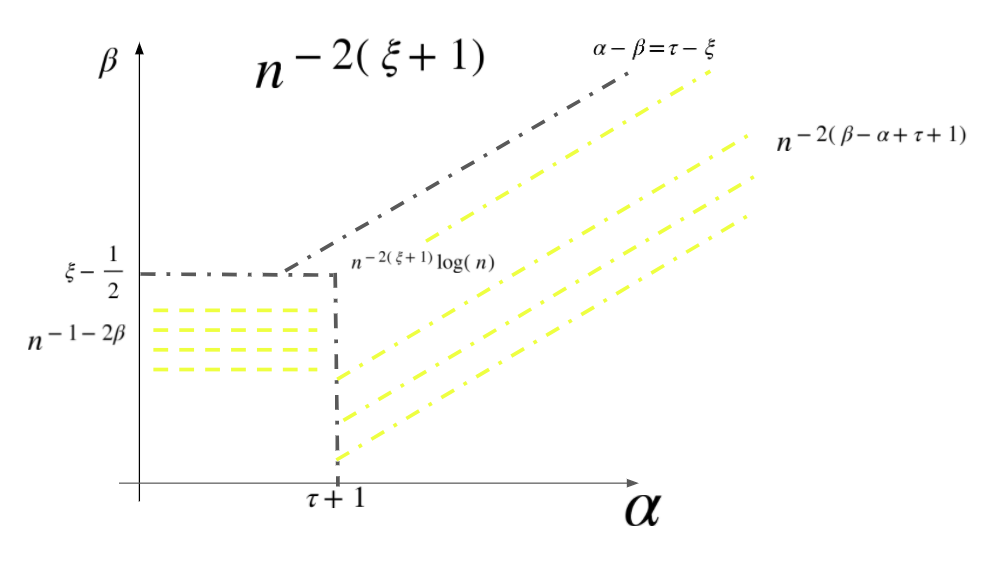
\includegraphics[width=10 cm]{imgs/diagram.PNG}
    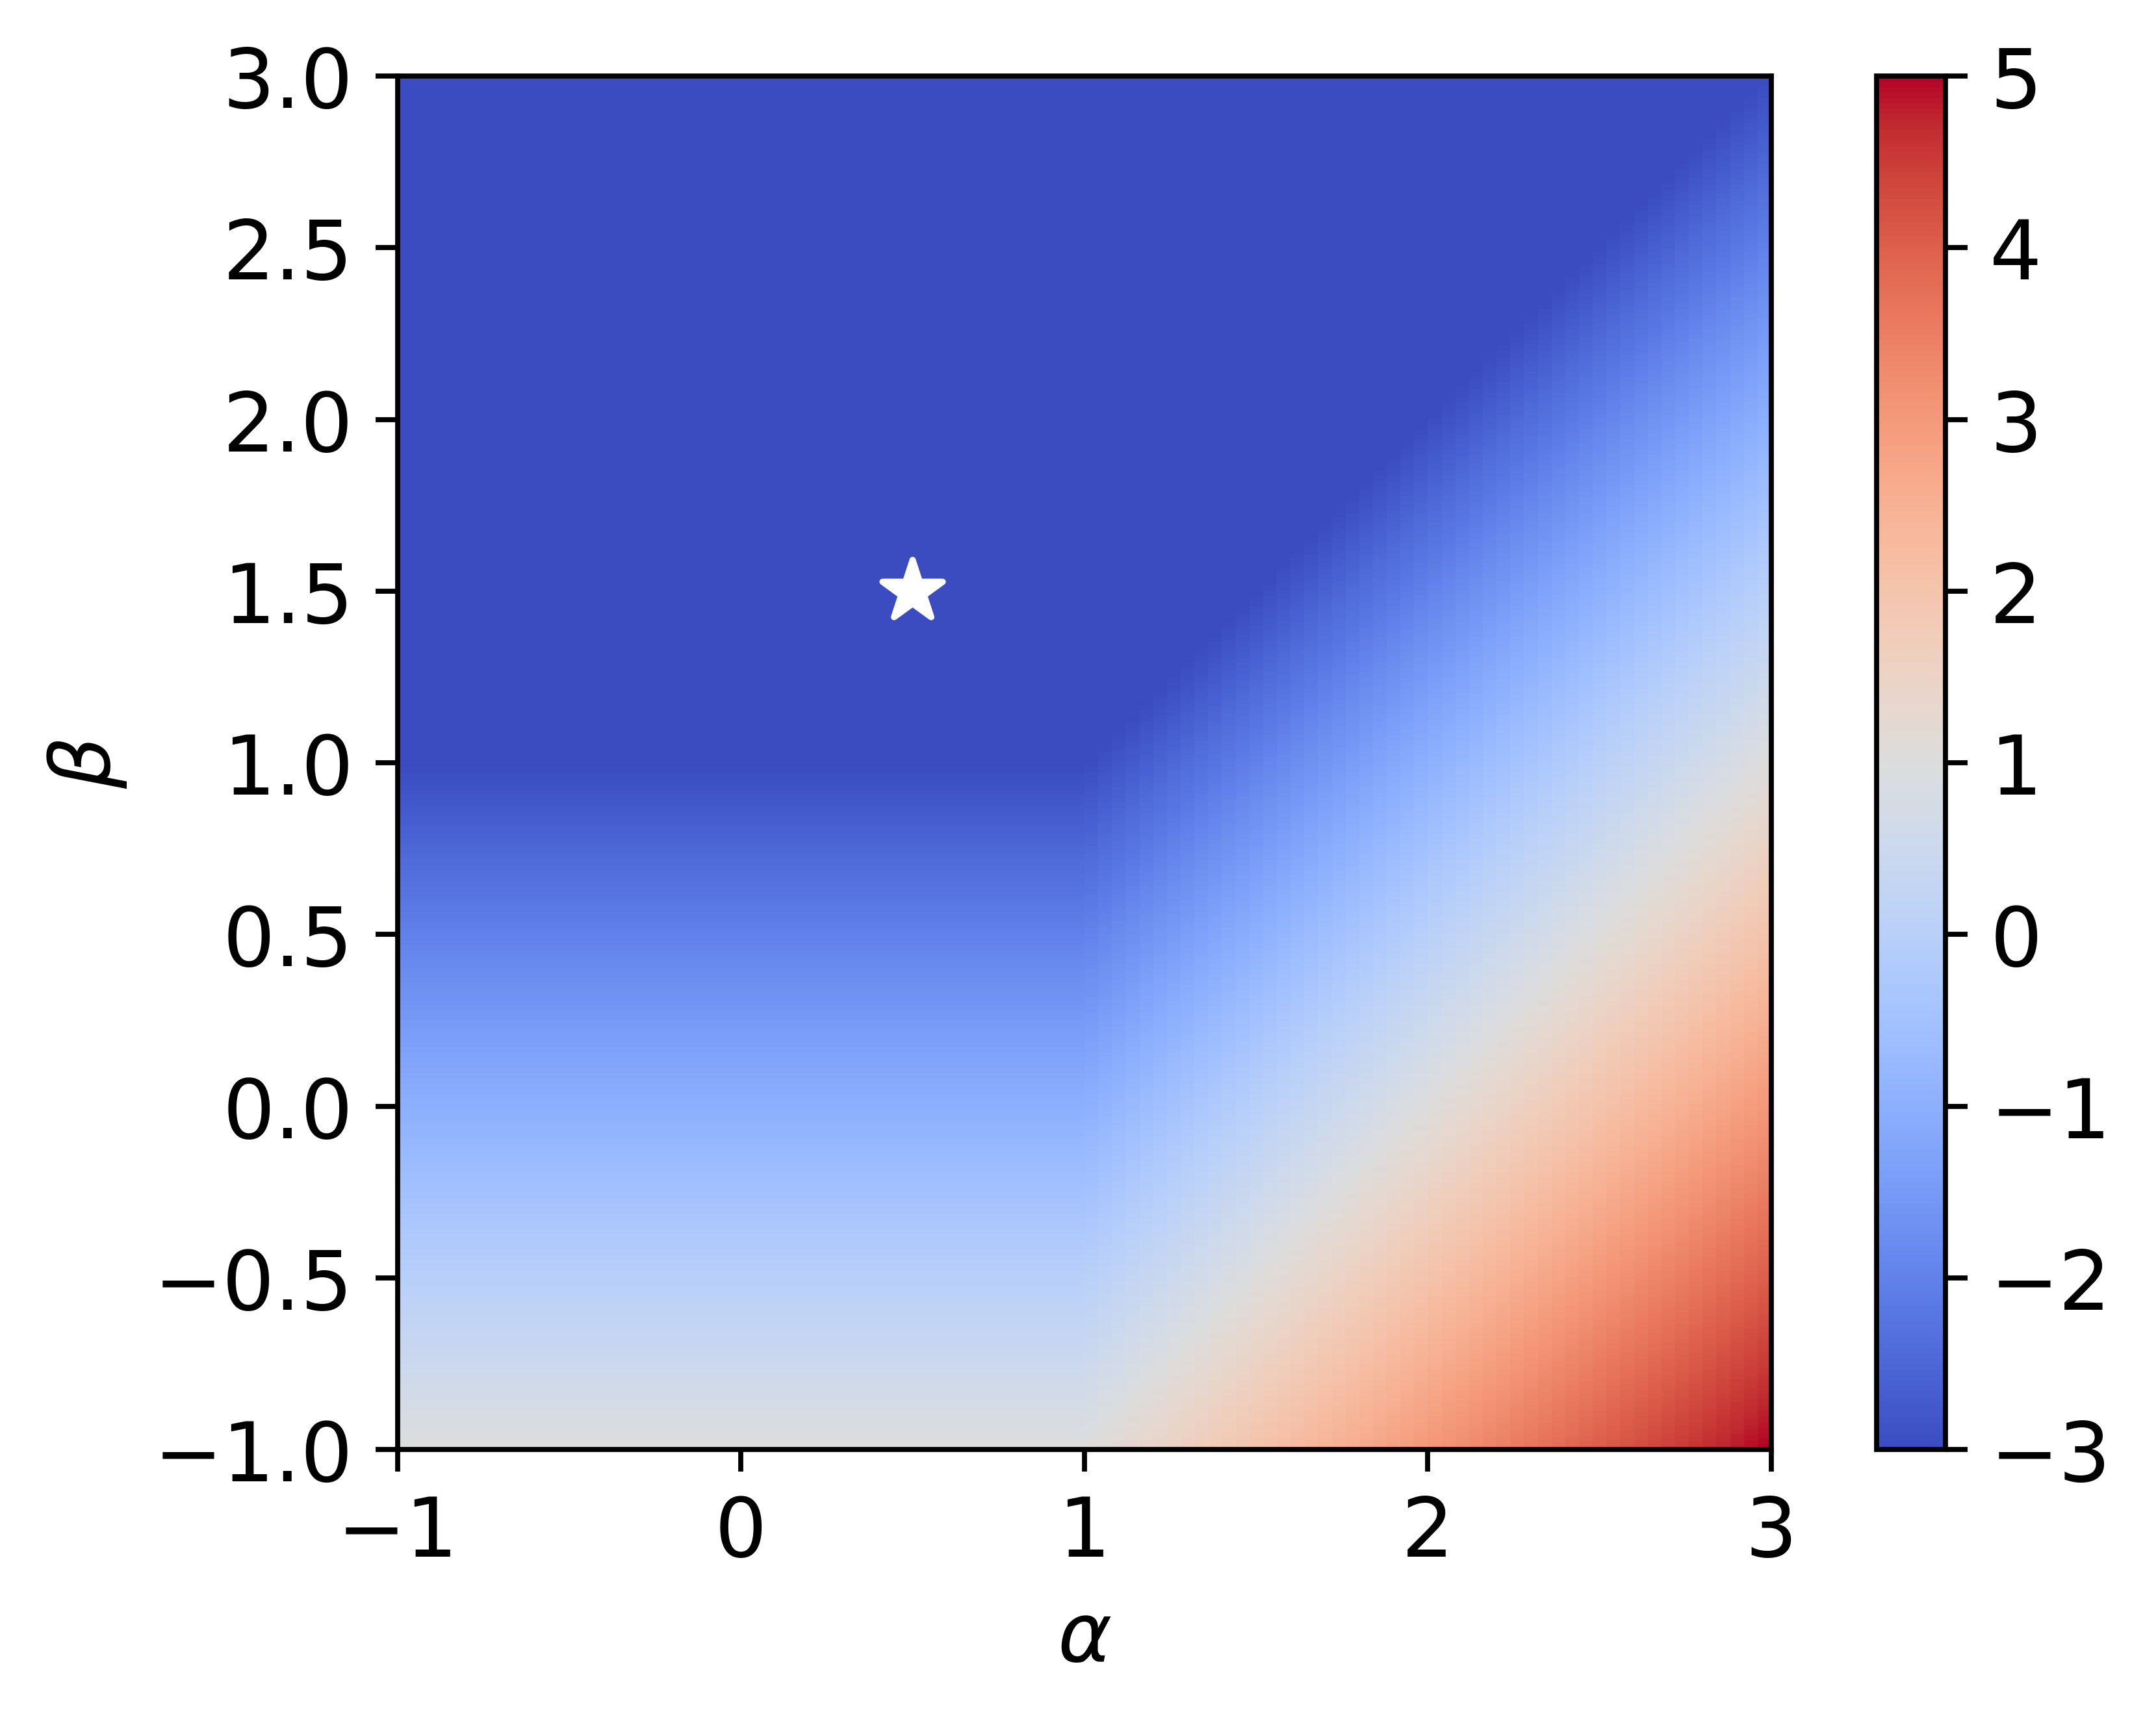
\includegraphics[width=0.4\textwidth]{new_imgs/cmap.png}
    \begin{small}
    \caption{Colormap for the function value average rates  for the Marchenko Pastur distribution and different tunings of the Generalized Chebyshev Method, $\alpha$ and. The white represents the optimal tuning, and the color represents the exponent, e.g. 'cooler' is better.}
    \end{small}
    \vspace{-2 cm}
\end{wrapfigure}


For the function value ($l=1$), we find rates that approach $t^{-2}$ as $\xi\rightarrow -1$, showing the worst-case as a limit (over the considered distribution) on the average case.
\begin{comment}


\begin{remark}
We can contextualize our results on the field of orthogonal polynomials as asymptotics on the values of the \textit{Christoffel Functions} at $0$ \citep{totik2005orthogonal}:

\begin{equation}
    \lambda_t(\mu,x)=\inf_{P_t(x):=1,\deg(P_t)\leq t}\int P_t^2 d\mu=\Big( \sum_{k=0}^tp_k(x;\mu)^2\Big)^{-1}
\end{equation}
 For the equivalence classes $\nu_{\tau,\xi}$
\end{remark}
\end{comment}
We remark that the above theorems imply that, at least asymptotically, the Jacobi method is robust for a suboptimal choice of parameter $\beta$ up to $1/2$ below the optimal choice and infinitely above. 


For completeness, we also derive worst-case rates for the Jacobi method:
\vspace{1.5 cm}

\begin{restatable}{prop}{worstcase}
Let $f$ be a convex, L-smooth quadratic function. Then, for the Generalized Chebyshev Method with parameters $(\alpha,\beta)$, we have:
\begin{align}
 f(\xx_t)-f(\xx^\star) \leq C_1L\left\{
    \begin{array}{cc}
           t^{2(\alpha-\beta)} &\text{if} \hspace{0.5 cm} \alpha>\beta-1 \\
         t^{-1-2\beta}, \hspace{1 cm} &\text{if} \hspace{0.5 cm} \alpha\leq \beta-1\hspace{0.5 cm} \beta\leq \frac{1}{2}\\
         t^{-2}, \hspace{1 cm} &\text{if} \hspace{0.5 cm} \alpha\leq\beta-1\hspace{0.5 cm} \beta\geq \frac{1}{2} 
    \end{array}
    \right . ,\\
    ||\nabla f(\xx_t)-f(\xx^\star)||\leq C_2L^2\left\{
    \begin{array}{cc}
           t^{2(\alpha-\beta)} &\text{if} \hspace{0.5 cm} \alpha>\beta-2 \\
         t^{-1-2\beta}, \hspace{1 cm} &\text{if} \hspace{0.5 cm} \alpha\leq \beta-2\hspace{0.5 cm} \beta\leq 3/2\\
         t^{-4}, \hspace{1 cm} &\text{if} \hspace{0.5 cm} \alpha\leq\beta-2\hspace{0.5 cm} \beta\geq 3/2
    \end{array}.
    \right. 
\end{align}
\end{restatable}


For  a reasonable choice of $\alpha,\beta$, i.e. $\beta\geq \frac{1}{2}$, $\alpha\leq \beta-1$. the function value achieves the theoretical lower bound of $t^{-2}$.

We now analyse the convergence of the Nesterov method. \cite{nesterov2003introductory} has shown that it matches up to a a constant factor a lower bound on the worst-case complexity of non strongly convex problems. A natural question is if this performance would translate to good average case rates. To do so, we will extend \citet{paquette2020halting} proof for the Nesterov method under the MP distribution.  
\begin{restatable}{theorem}{nesterovrates} \label{the: neste rates}
Let $\nu$ as in Assumption \ref{assumption}. Then for the Nesterov method
\begin{equation}
    \mathbb{E}[f(\xx_t)-f(\xx^\star)]\sim C'_{1,\nu}
    \Big\{\begin{array}{ll}
		  t^{-2(\xi+2)}& \mbox{if } 
		  \xi<-1/2\\
		  t^{-3}\log t& \mbox{if } 
		  \xi=-1/2\\
		  t^{-(\xi+7/2)}& \mbox{if } 
		  \xi>-1/2
	\end{array}, \hspace{1 cm}
	\mathbb{E}[||\nabla f(\xx_t)||^2_2] \sim C'_{2,\nu}
		  t^{-(\xi+9/2)}.
\end{equation}
\end{restatable}

The difference between the assymp. rates of Nesterov and the optimal ones are $t{\xi+l-1/2}$, when $\xi+l>1/2$, $\log t$ when $\xi+l=1/2$ and $0$ otherwise.
This shows that Nesterov is almost optimal when the concentrations near $0$ are relatively high, i.e. low $\xi$.

\begin{restatable}{theorem}{gdrates} \label{the: gd rates}
Let $\nu$ as in Assumption \ref{assumption}. Then for gradient descent
\begin{equation}
\mathbb{E}[f(\xx_t)-f(\xx^\star)]=\Theta(t^{-(\xi+2)}), \hspace{1 cm}
	\mathbb{E}[||\nabla f(\xx_t)||^2_2] =\Theta(t^{-(\xi+3)}).
\end{equation}

\end{restatable}

Observe for the function value that the rate for Nesterov is $t^{-2}$ and the rate for Gradient Descent is $t^{-1}$ when $\xi \rightarrow -1$. 
%we  find the $t^{-2}$ rates for Nesterov and $t^{-1}$ for Gradient Descent  when $\xi\rightarrow-1$

\begin{table}[t]
    \centering
    \begin{tabular}{c|c|c|c|c}
         $(\tau,\xi)$/Method& Chebyshev ($\frac{1}{2},\frac{5}{2}$) & Chebyshev ($\frac{1}{2},\frac{3}{2}$) &  Nesterov  & G.D. \\
         \hline
         ($\frac{1}{2},\frac{1}{2}$)&$t^{-5}$ & $t^{-4}$ & $t^{-4}$ & $t^{-\frac{5}{2}}$\\
         \hline
         ($\frac{1}{2},\frac{-1}{2}$)&$t^{-3}$ & $t^{-3}$ & $t^{-3}\log t$ & $t^{-\frac{3}{2}}$
    \end{tabular}
    \caption{Comparison of asymptotic rates for the function-value for different methods an $(\tau,\xi)$ values}
    \label{tab:theoretic rates}
\end{table}

Lastly, we consider the optimal rates for a Gamma distribution.

\begin{restatable}{theorem}{laguerrerates}
Let $\alpha>-1$ and $\mu_\alpha$ be a Gamma distribution, i.e. $d\mu_\alpha(x)=\frac{x^\alpha e^{-x}}{\Gamma(\alpha+1)}$. The optimal rates are given by the Laguerre method of appropriate tuning and
\begin{equation}
    \mathbb{E}[f(\xx_t)-f(\xx^\star)]=\Theta(t^{-(\alpha+2)}) . 
    %%we can get the constants here
\end{equation}
\end{restatable}
Note that this result does not have the same universality of the others because of the non-compacity of the distribution's support.

These rates are contrasted  to the worst-case lower bound on the optimization of non-smooth functions by first-order methods, which gives
\begin{equation*}
    f(\xx_k)-f(\xx^\star)\geq\frac{C}{\sqrt{t}} .
\end{equation*}
These rates are not found when $\alpha\rightarrow-1$, indicating that the worst-case is especially pessimistic in this scenario.


\section{Experiments}

We simulate the e.s.d's  in two ways. The Marchenko Pastur distribution, which we sample by taking $H=\XX\XX^T$ where $\XX$ has i.i.d samples, that enables us to simulate $(\tau,\xi)$ values of $(1/2,3/2)$ and $(1/2,5/2)$. 

Other values of $(\tau,\xi)$ are simulated by sampling $\Lambda \in \RR^d$ from the corresponding Beta distribution and taking $\HH=\UU\diag(\Lambda)\UU^T$, where $\UU$ is an independently sampled orthonormal matrix. 

We let $\xx^\star=0$ and sample $\xx_0$ from a centered gaussian distribution, the dynamics are the same as in the general case

%Because we work with the asymptotic rates on the infinite dimensional case, i.e. we take $d\rightarrow \infty$ and then $t \rightarrow \infty$, they are representative of the experiments on the regime $t<d$.

Our theoretical rates in theorems \ref{the: gd rates} \ref{the: neste rates} for the Nesterov method and Gradient Descent are precise under the approximate  range $-1<\xi<0$  as we show in figure \ref{fig: last figure}. Distributions with higher $\xi$ need many samples otherwise they behave as strongly convex functions. 

The same is not true for the Generalized Chebyshev Method. If $\beta<\beta^\star$ or $\xi$ is low the empirical findings diverge from the theoretical. We believe this is due to numerical instability under these regimes as the metrics also have  much larger variance than in the other regimes. This shown in appendix \ref{appendix: experiments}.  

The GCM with  $\beta>\beta^\star$ perform corresponding to the theory, and it's non-asymptotically very close to the performance of $\beta^\star$. High values of $\beta$ also perform very well on non-synthetic data, suggesting in practice we should use these values.

\begin{figure}[h]
    \centering
    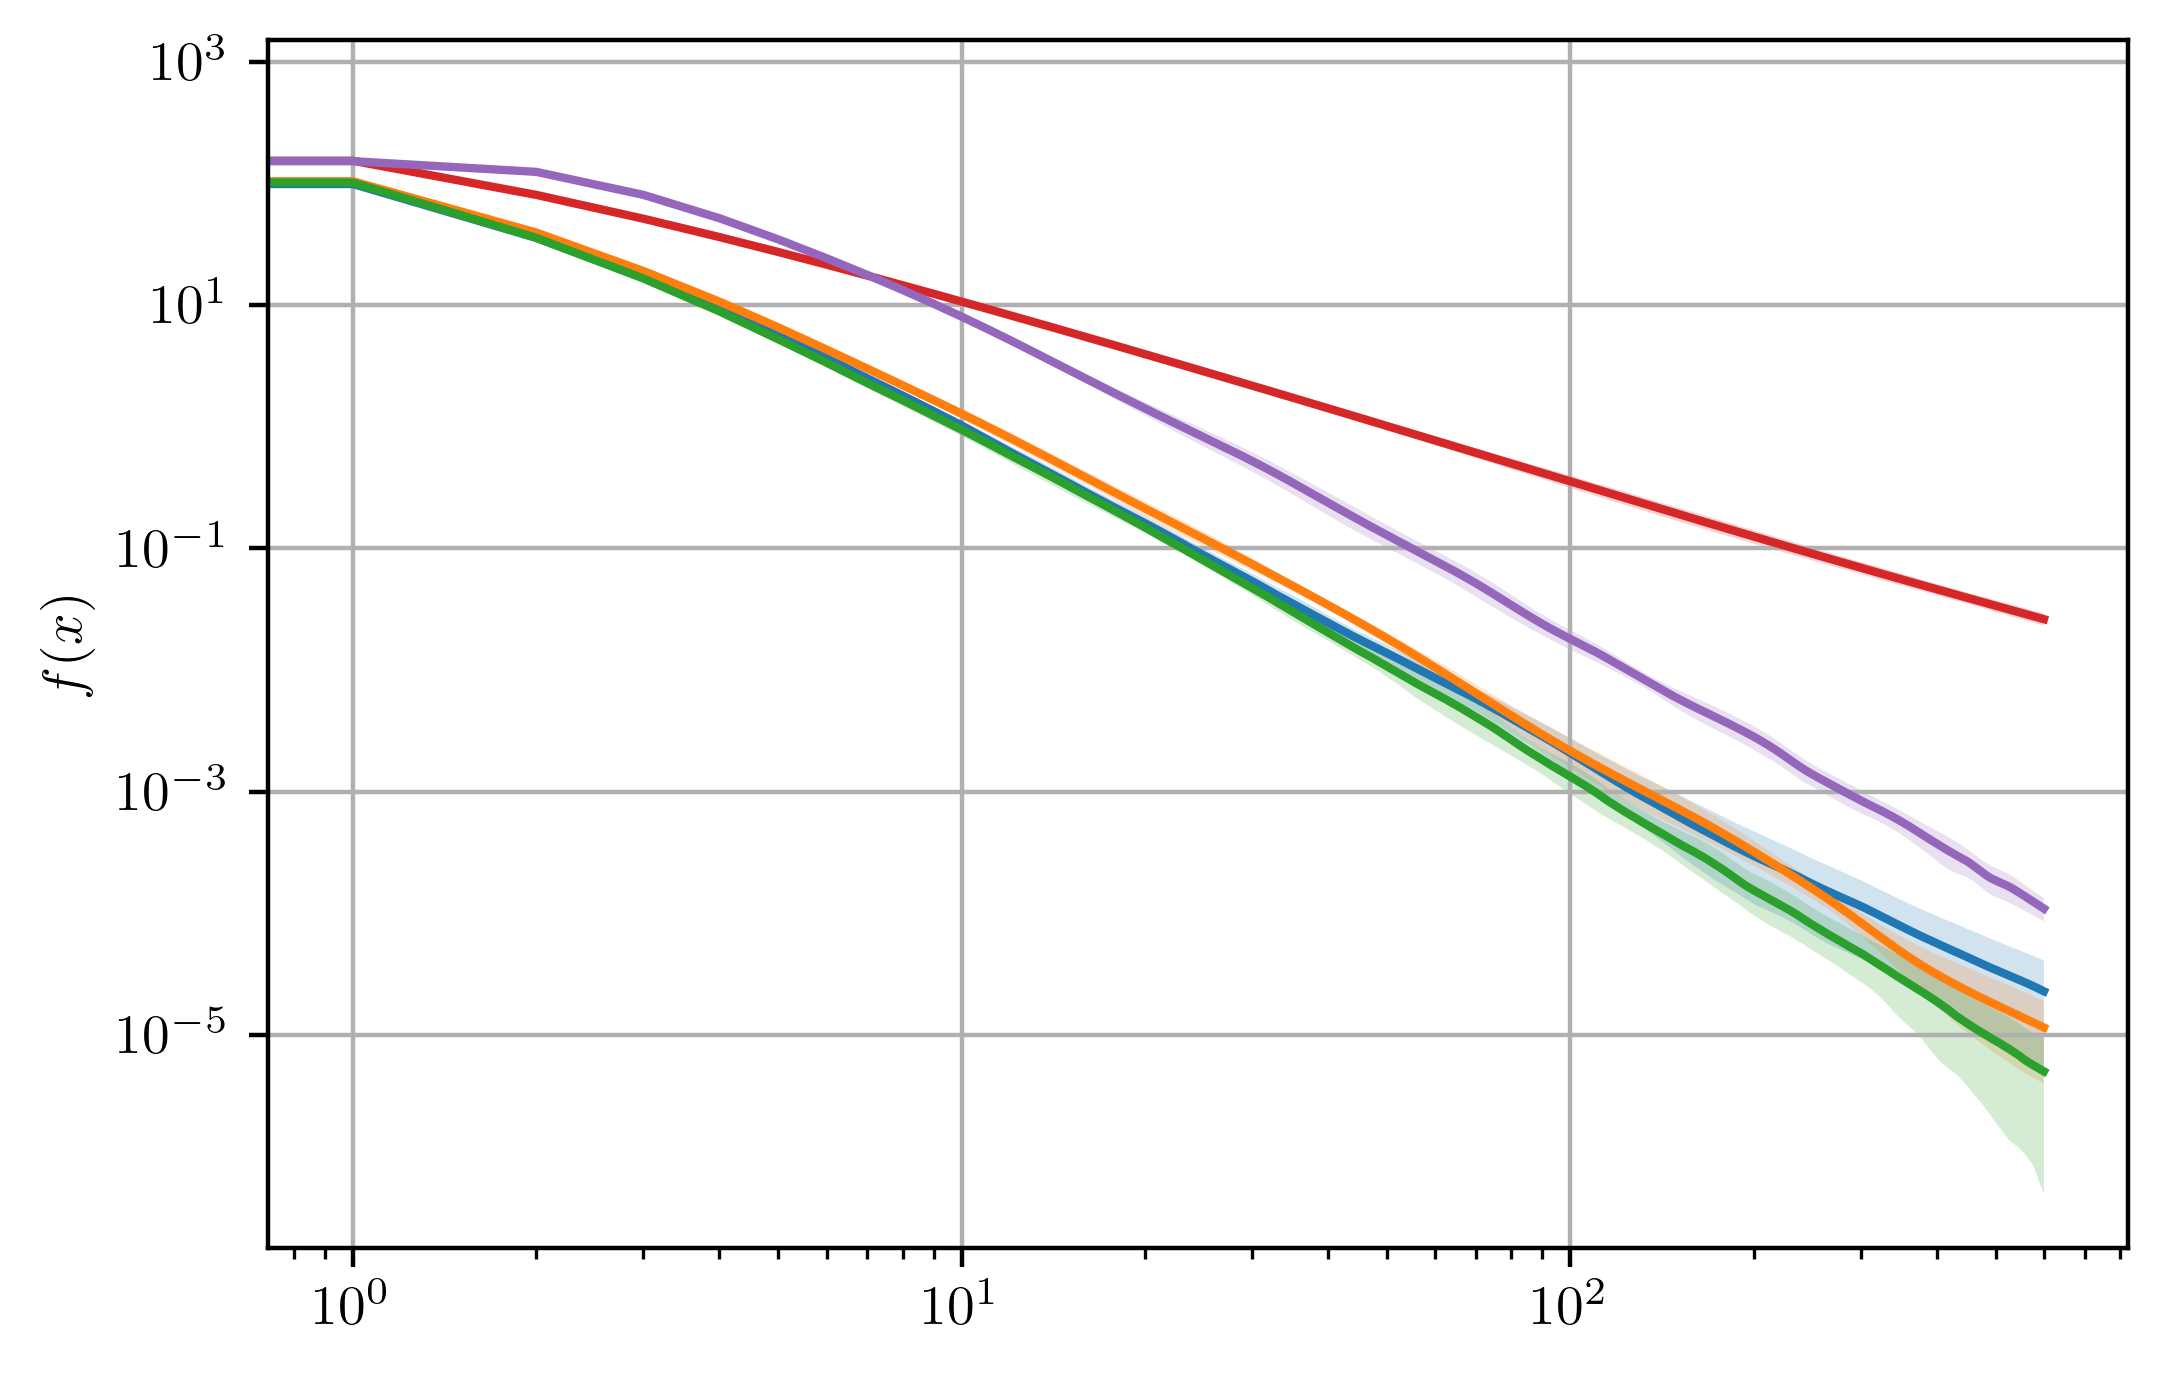
\includegraphics[width=5 cm]{new_imgs/mp f.png}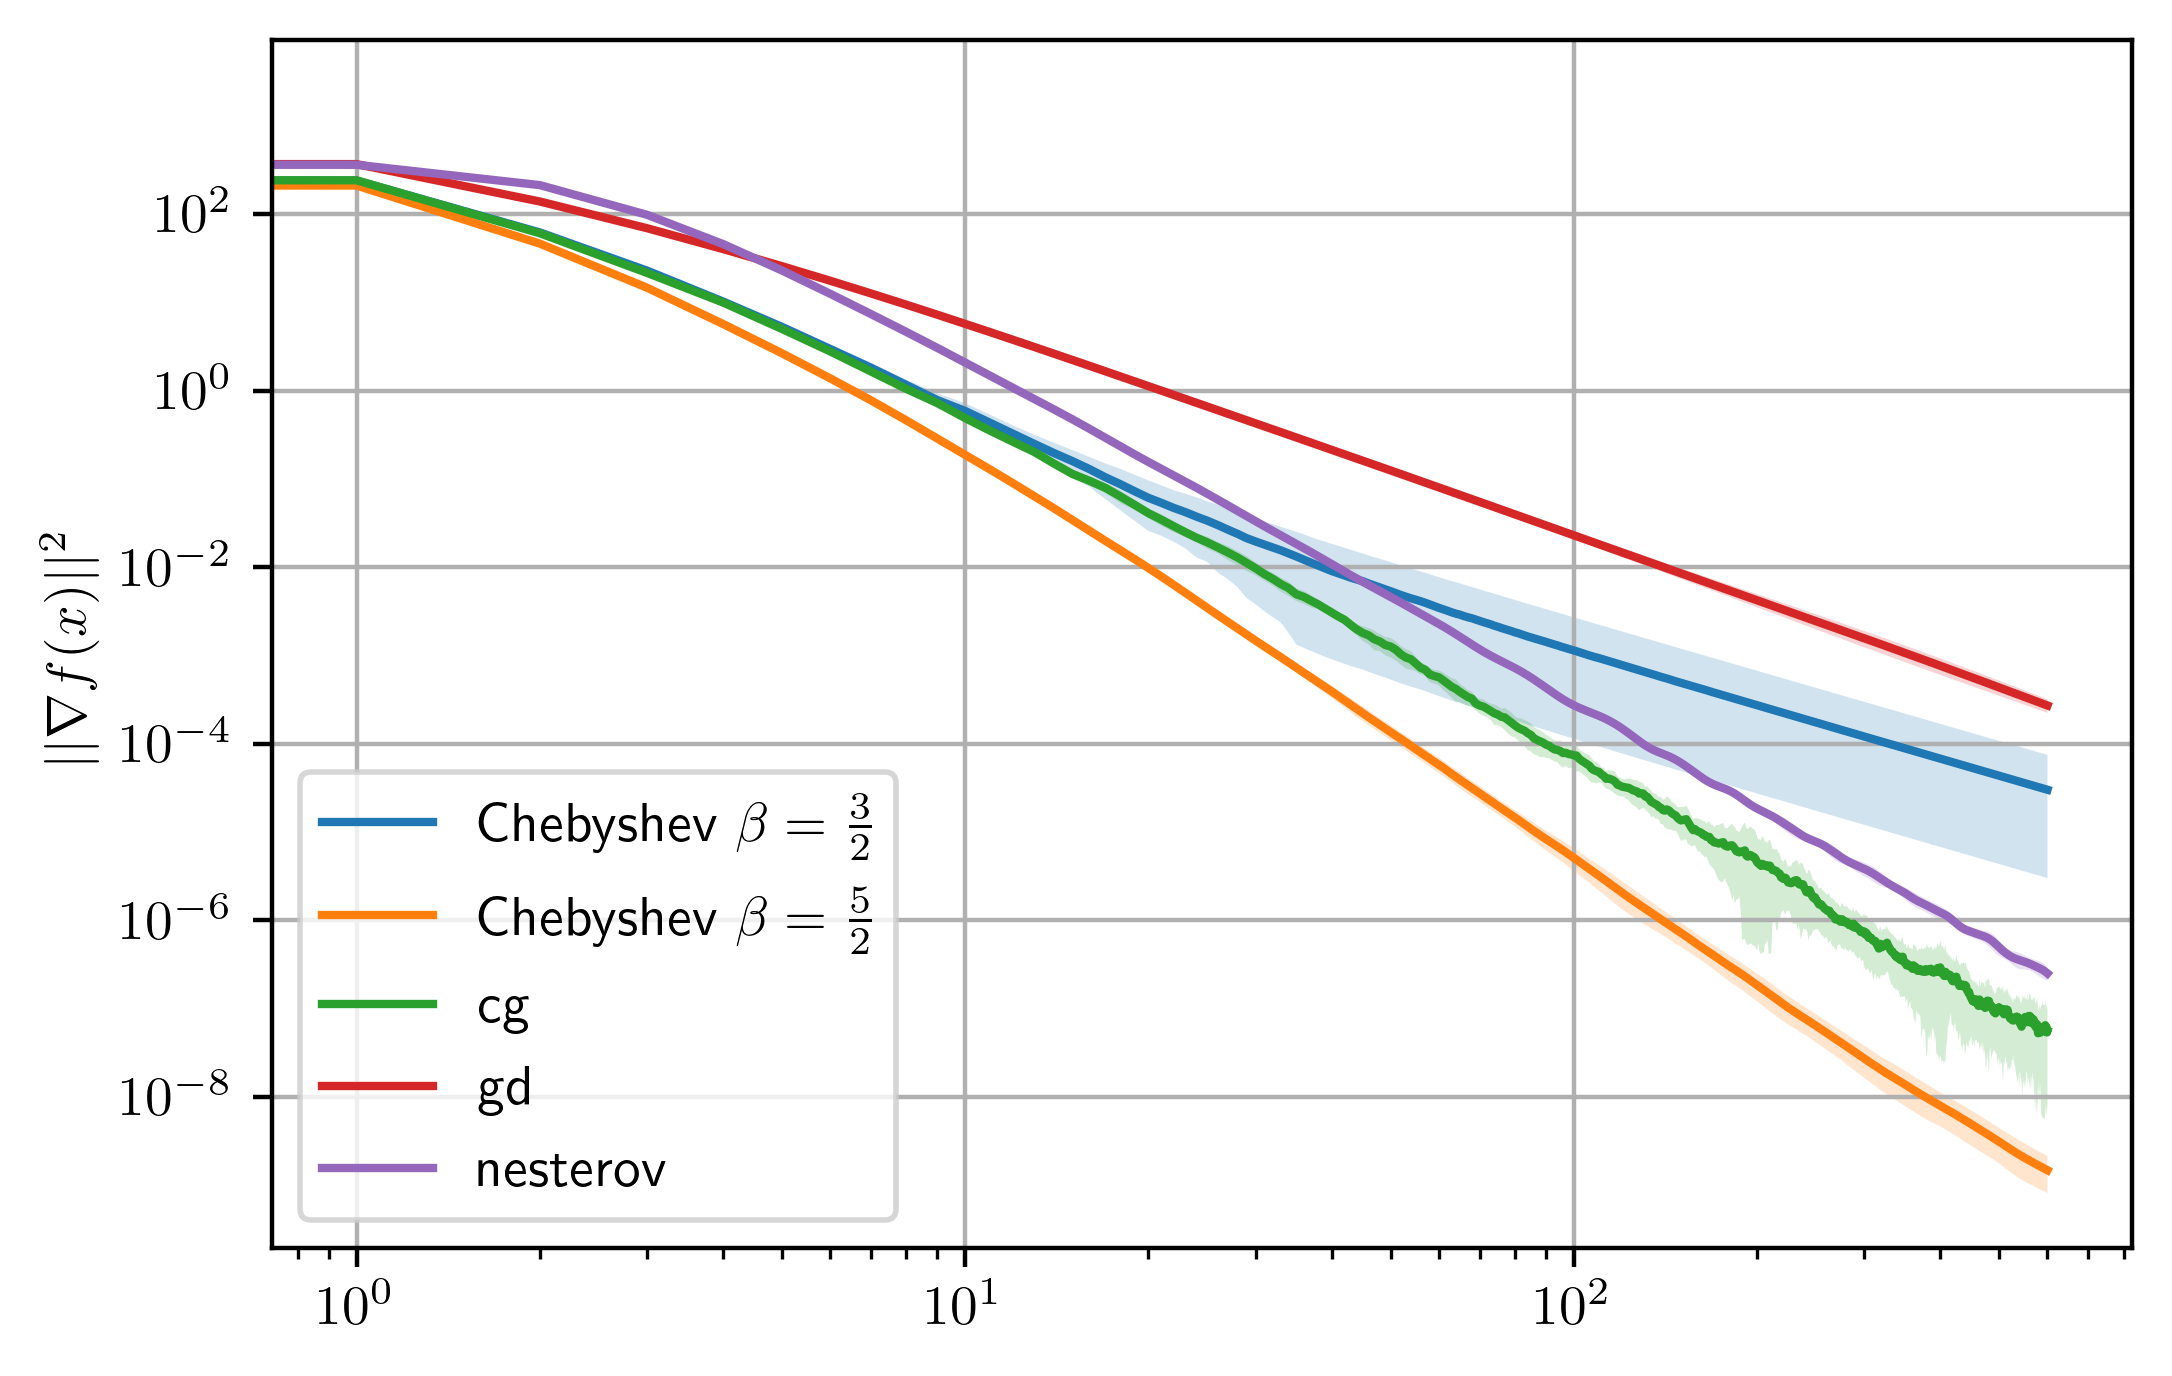
\includegraphics[width= 5 cm]{new_imgs/mp grad.png}
    
    
    \caption{Rates for a synthetic problem, simulating the Marchenko Pastur distribution. Note that both tunings of the GCM achieve performance in function value very close to the one of Conjugate Gradient, which is optimal for every draw of the problem.}
    \label{fig:my_label}
\end{figure}

\begin{figure}[h]
    \centering
    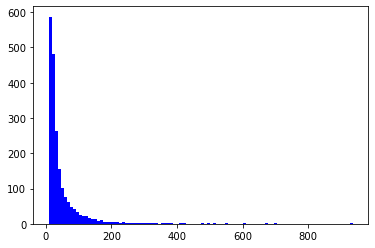
\includegraphics[width=5 cm]{imgs/inception/spectrum.png}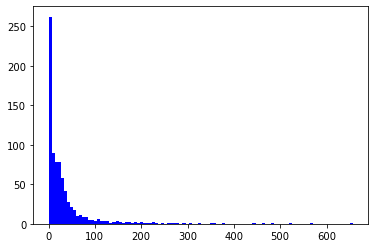
\includegraphics[width= 5 cm]{imgs/mnist/spectrum.png}
    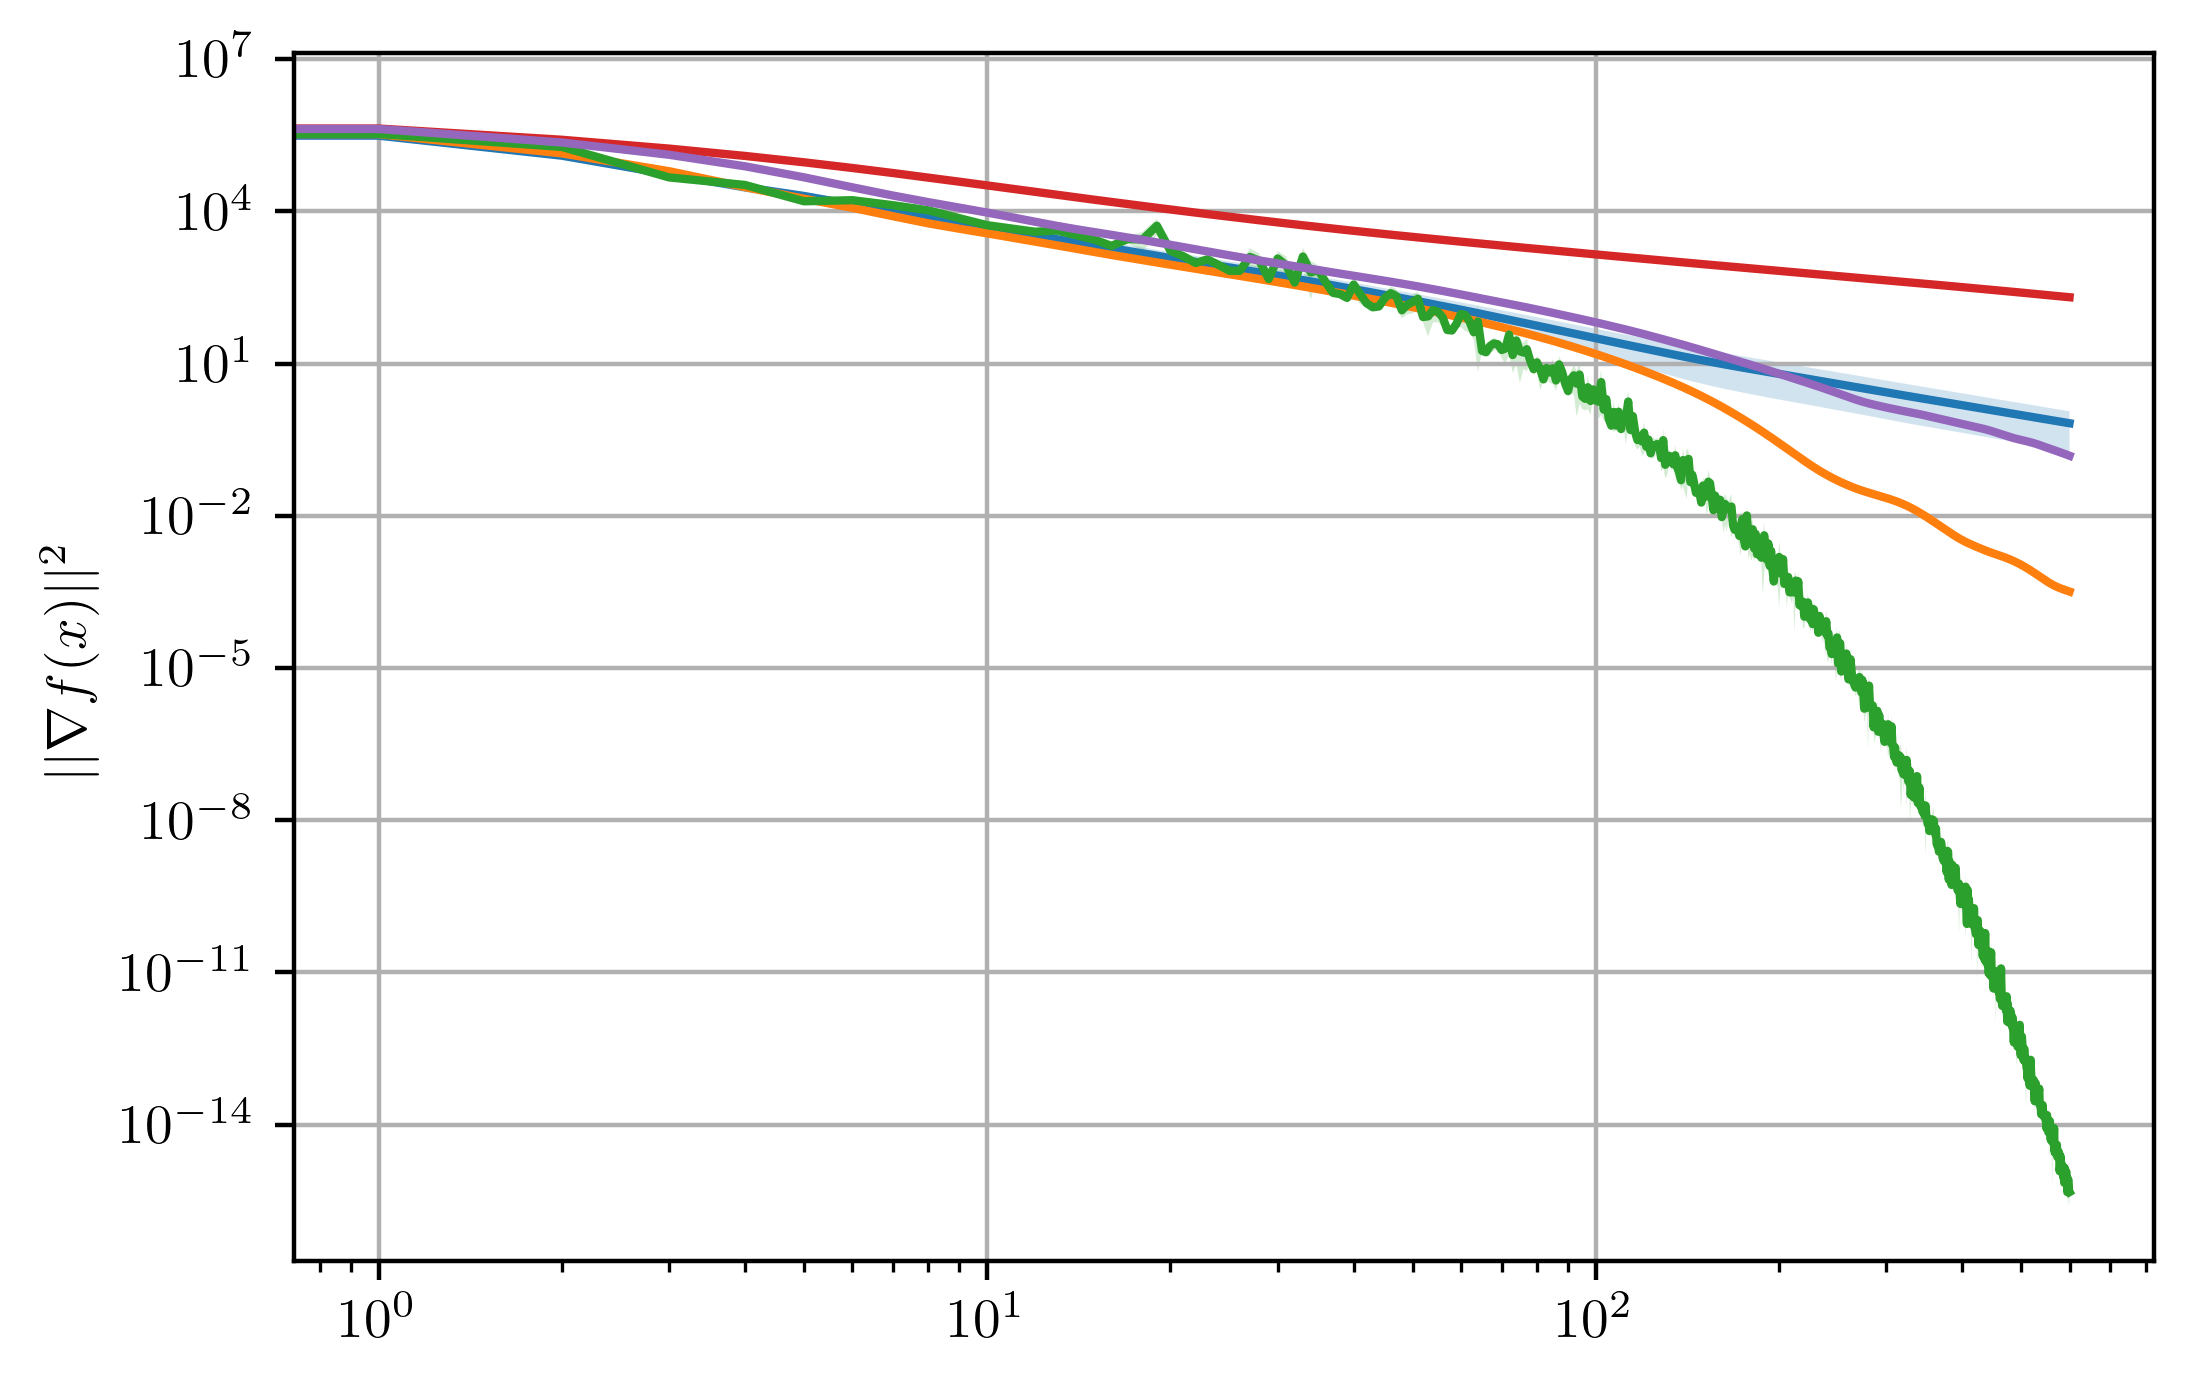
\includegraphics[width=5 cm]{new_imgs/inception.png}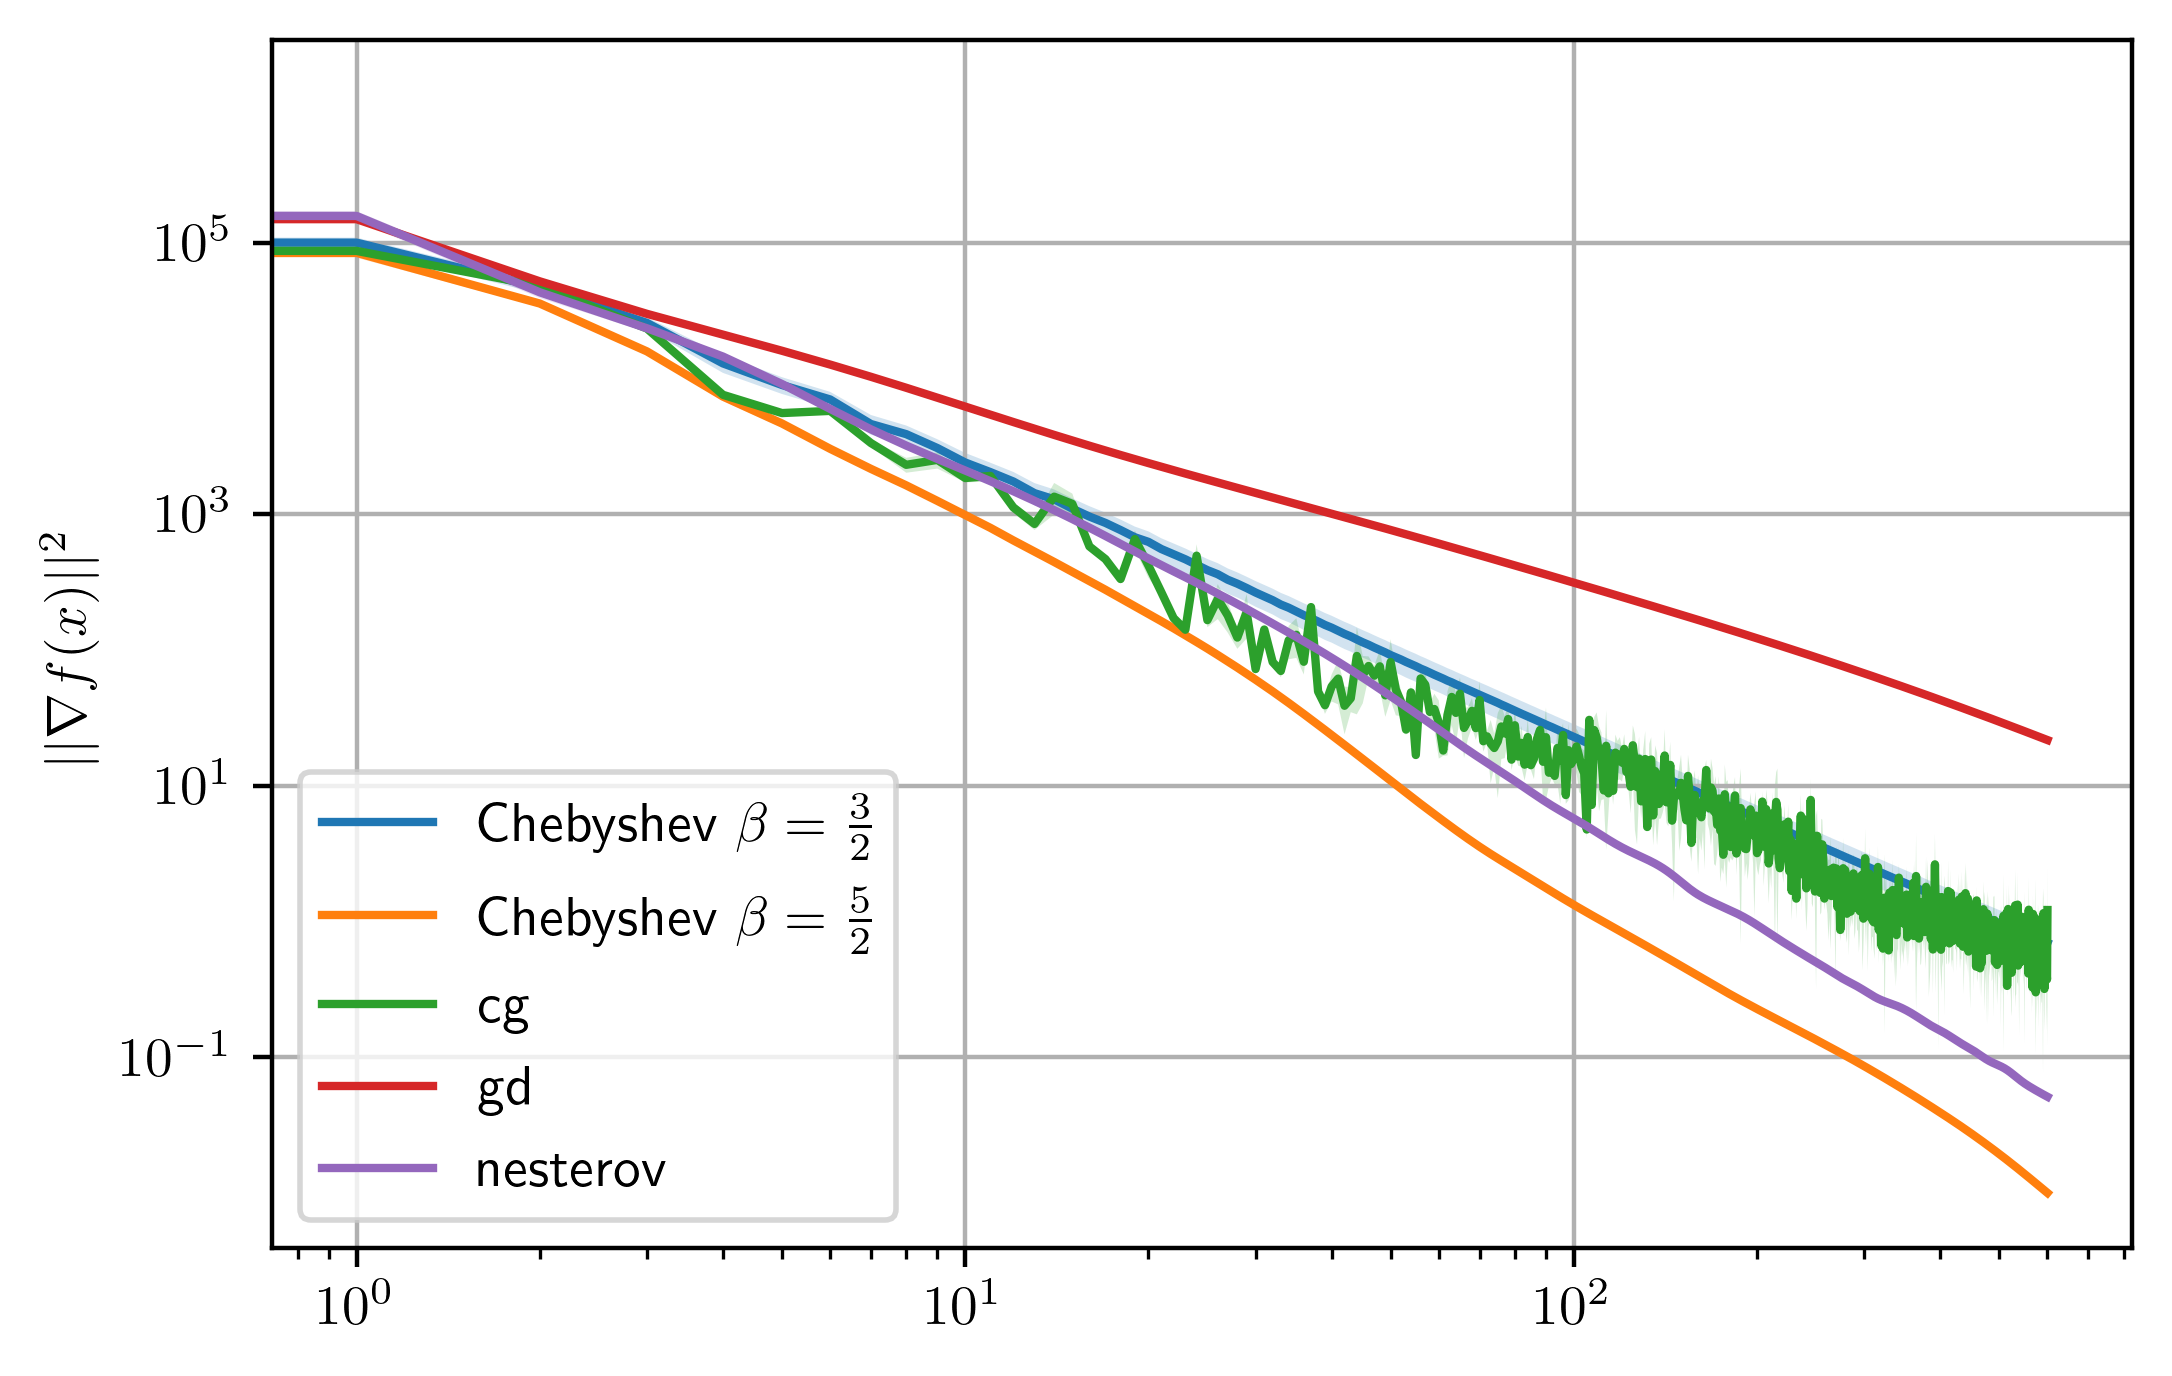
\includegraphics[width= 5 cm]{new_imgs/mnist.png}
    
    
    \caption{Spectrum and gradient norm rates for regression problems. \textit{Left:} CIFAR-10 Inception features \textit{Right}: MNIST features. Here we choose to compare gradient norms as the minimum function value is not known. The properly tuned GCM achieves remarkable performance under these non-synthetic spectrum's.
}
    \label{fig:my_label}
\end{figure}


\begin{comment}
\begin{table}[H]
    \centering
    \begin{tabular}{c|c|c|c}
         $(\tau,\xi)$/Method& Chebyshev ($\frac{1}{2},\frac{5}{2}$) & Chebyshev ($\frac{1}{2},\frac{7}{2}$) &  Nesterov  \\
         \hline
         ($\frac{3}{2},\frac{1}{2}$)&$t^{-3.96}$? & $t^{-4.93}$ & $t^{-4.01}$\\
         \hline
         ($\frac{1}{2},\frac{1}{2}$)&$t^{-3.00}$ & $t^{-2.83}$ & $t^{-2.68}$
         
    \end{tabular}
    \caption{Empirical slopes for the function-value }
    \label{tab:experimental rates}
\end{table}
\begin{figure}[h]
    \centering
    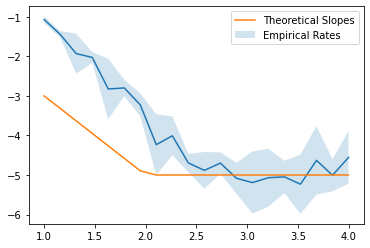
\includegraphics[width=5 cm]{imgs/theo vs practic.png}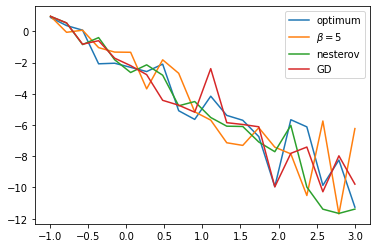
\includegraphics[width= 5 cm]{imgs/slopes.png}
    
    
    \caption{Left: Empirical vs theoretical rates for fixed $\xi$ and varying $\beta$. Right: Empirical slopes for varying $\xi$}
    \label{fig:my_label}
\end{figure}

\end{comment}








\begin{figure}[H]
    \centering
    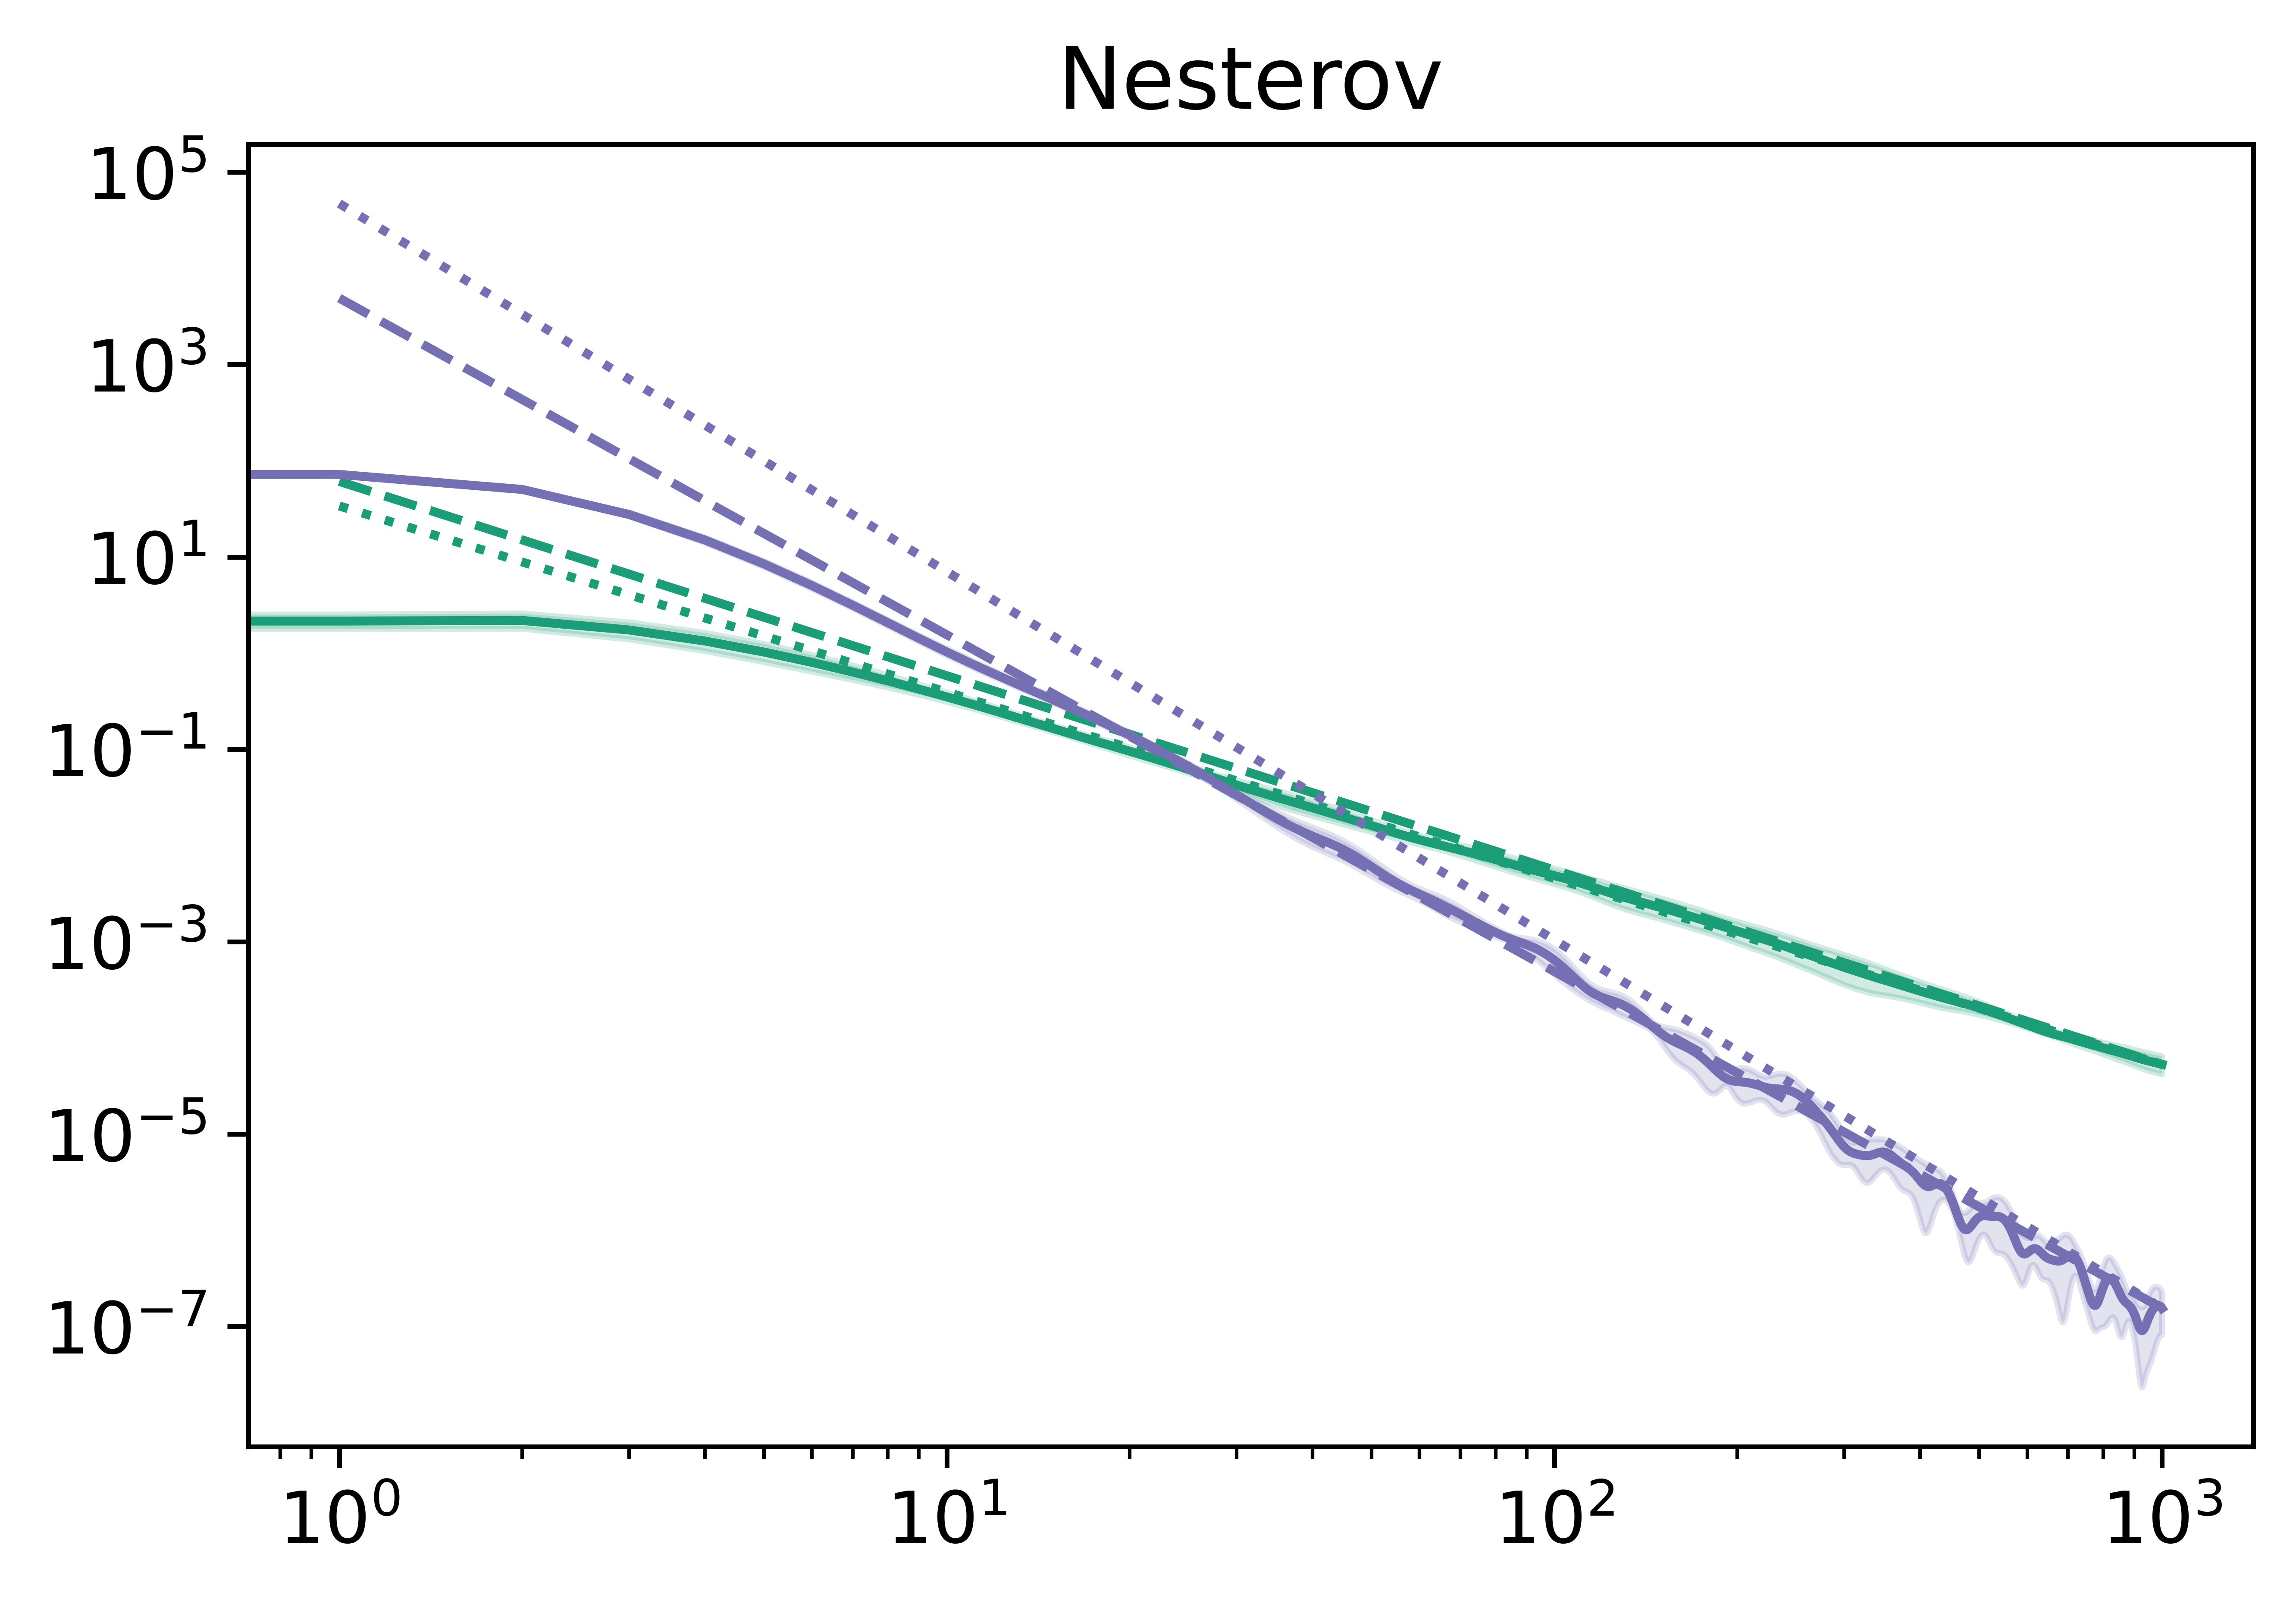
\includegraphics[width= 0.4\textwidth]{new_imgs/nesterov.png}
    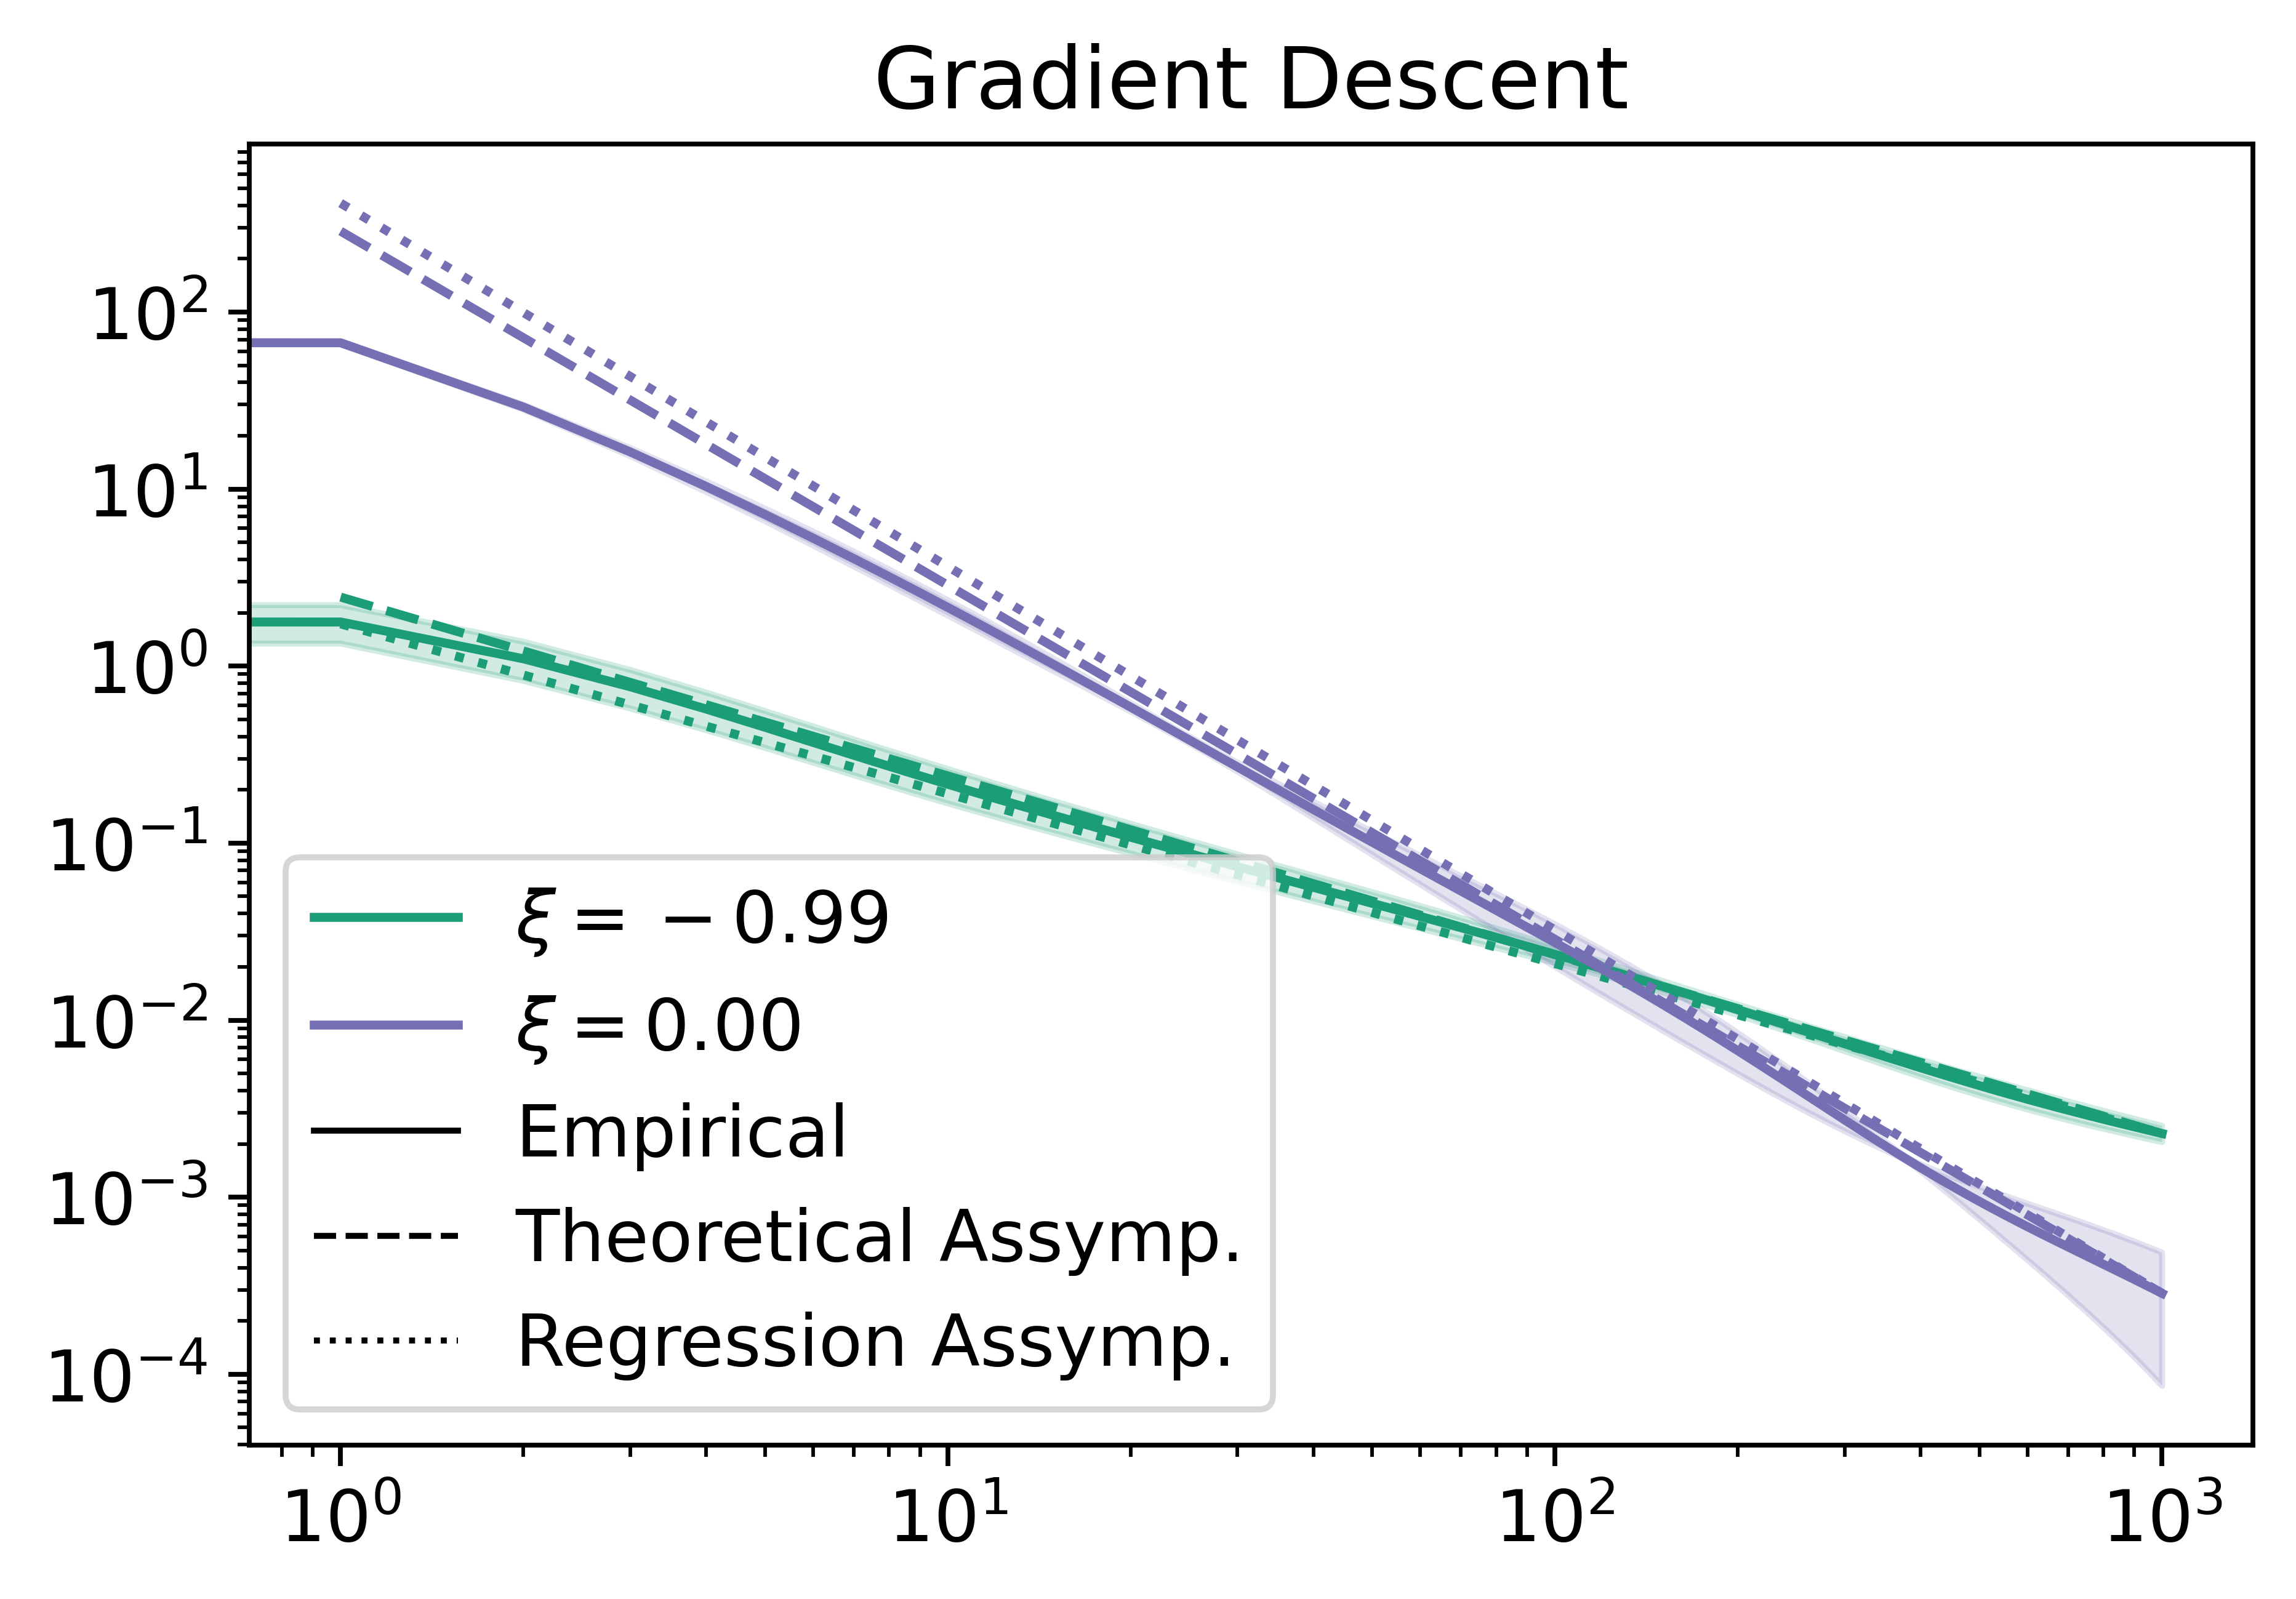
\includegraphics[width= 0.4\textwidth]{new_imgs/GD.png}\\
        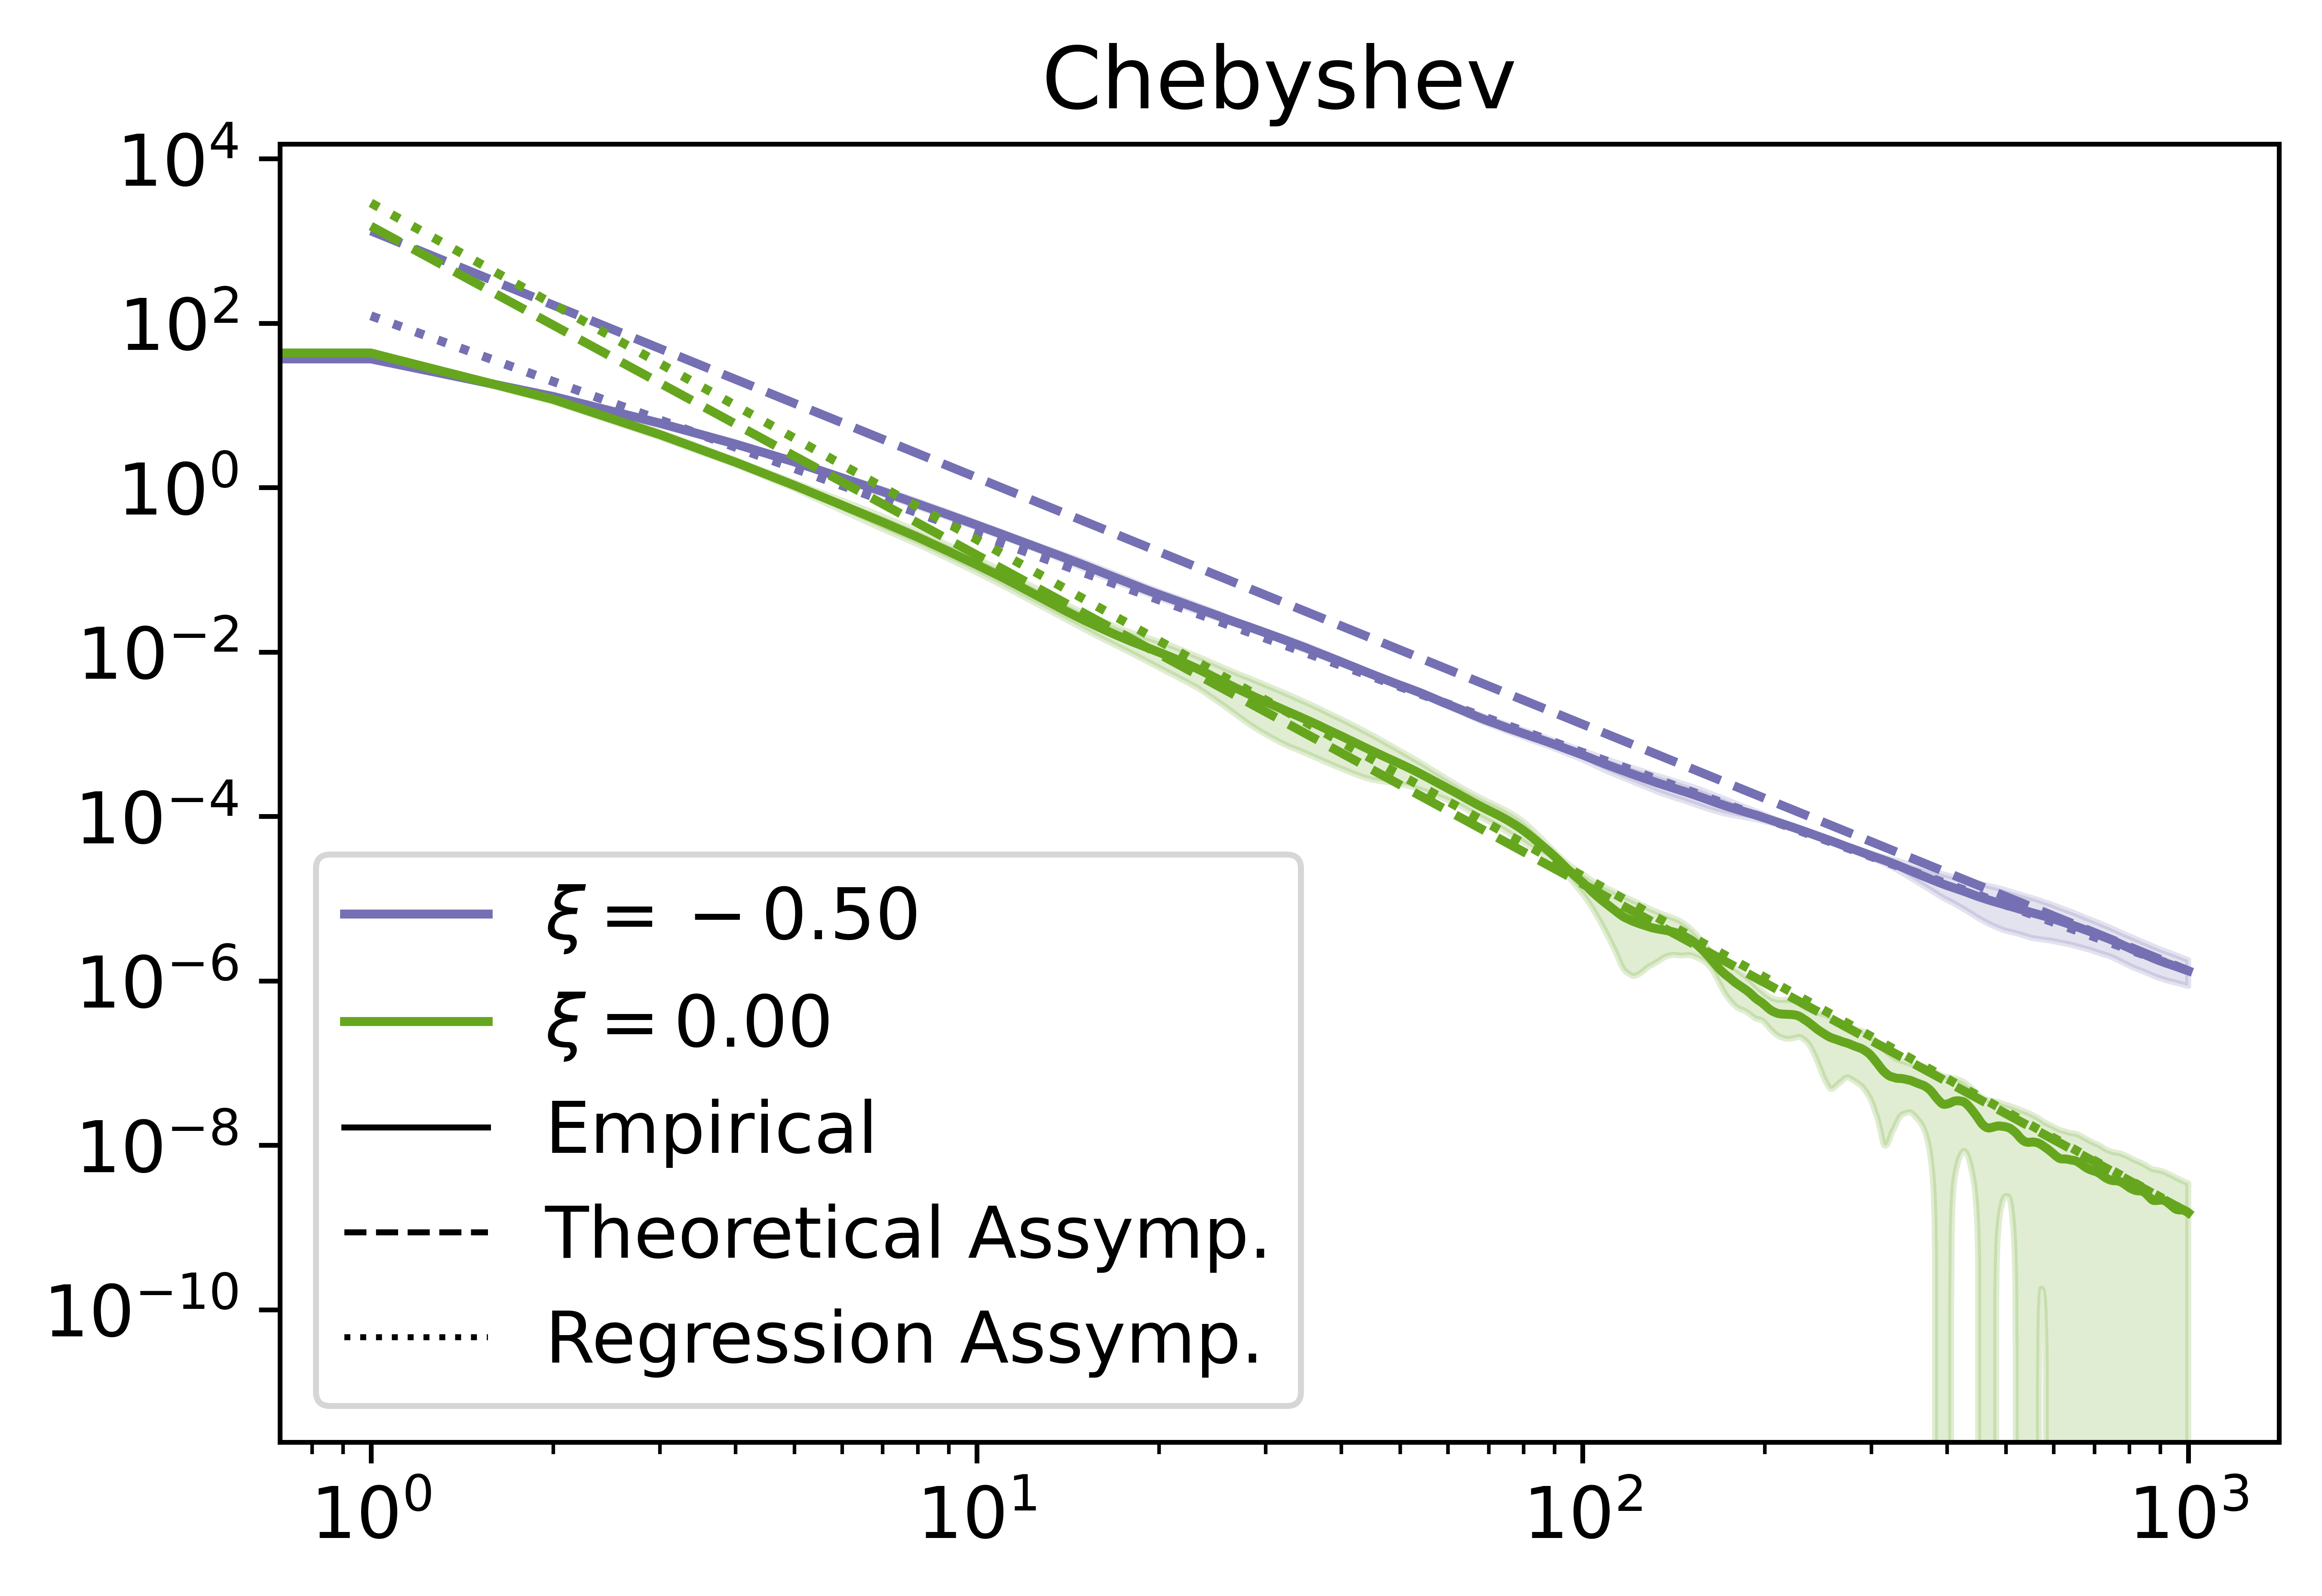
\includegraphics[width= 0.4\textwidth]{new_imgs/chebyshev.png}

    \caption{Comparison between experiments run on synthetic Beta distribution and theoretical asymptotic. Y-axis is function value }
    \label{fig: last figure}
\end{figure}


%%Chebyshev \beta=5/2 is not giving the expected gradient performance ...


\section{Conclusion}
From a practical standpoint, we have proposed the Generalized Chebyshev method which shows remarkable performance on real world datasets. 

From a theoretical standpoint, we've shown the Nesterov method, which is easier to implement and more numerically stable, to be very close to the asymptotic optimum   under some natural assumptions over the data, namely a concentration of eigenvalues around $0$ similar to the Marchenko-Pastur measure. This adds to the theoretical understanding of why Nesterov acceleration is such a good method in practice. 

We have  shown that the average case asymptotic convergence of  the better known f.o.m. depend only on the concentrations of the problem's eigenvalue near the edges. We have shown these rates to be representative of the practical performance of the algorithms, and retrieve the classical worst-case rates as limits of the average case

Finally, we have characterized the optimum average case convergence under the scenarios analogous to the three usual hypothesis in worst-case convergence analysis which we resume in table \ref{table: rates}.

We consider analysing the Generalized Chebyshev methods and the average convergence in problems beyond quadratics minimization the main follow-up direction to our work. We conjecture one can show local convergence, and local average case rates, for general convex functions by a similar method to \cite{wang2021modular}, which has shown the size of the convergent neighborhood for the Polyak method for general strongly convex smooth functions.
\newpage
\bibliography{citations.bib}
\bibliographystyle{ICLR/iclr2022_conference}

\appendix
\newpage
\section{Proofs of Section \ref{section: average case}}
\metrics*
\begin{proof}
\newcommand\xinit{\xx_0-\xx^\star}
We remark that by the definition of the expected spectral distribution $\mu$ of $\HH$, we have for continuous $g$
\begin{equation}
    \EE_H[g(tr(\HH))]=\int g(\lambda)\dif \mu(\lambda) 
\end{equation}
We know that $\xx_t-\xx^\star=P_t(\HH)(\xinit)$. We can write $||\xx_t-\xx^\star||^2$ in terms of a trace and use the independence of $\HH$ and $\xinit$ to connect it to the e.s.d.:
\begin{align}
    \mathbb{E}||\xx_t-\xx^\star||^2&=\EE[ tr((\xinit)^TP_t(\HH)^2(\xinit))] \\
    &=\EE_{\HH,\xinit} [tr(P_t(\HH)^2(\xinit)(\xinit)^T]\\
    &=\EE_\HH\left[P_t(\HH)^2\EE_{\xinit}[(\xinit)(\xinit)^T])\right]  \\
    &=R^2\EE_\HH[P_t(tr(\HH))^2]=R^2 \int P_t(\lambda)^2\dif\mu(\lambda)
\end{align}
For the gradient and function value the reasoning is the same by noticing that
\begin{align}
    \EE[f(\xx_t)-f(\xx^\star)]&=\EE[ tr((\xinit)^TP_t(\HH)\HH P_t(\HH)(\xinit))]\\
    &=\EE_\HH[(\lambda P_t)(\tr(H))^2],
\end{align}
where $\lambda P_t$ is also a  polynomial. As $\nabla f(\xx_t)=\HH(\xx_t-\xx^\star)$.
\begin{align}
    \EE||\nabla f(\xx_t))||^2&=\EE[ tr((\xinit)^TP_t(\HH)\HH^2 P_t(\HH)(\xinit))]\\
    &=\EE_\HH[(\lambda^2 P_t)(\tr(H))^2]
\end{align}


\end{proof}

\optimality*
\begin{proof}
We differentiate the expression for the metrics w.r.t. to the coefficients of the polynomials:
\begin{align*}
    \frac{d}{da_k}\left(\int \lambda^lP_t^2(\lambda)d\mu(\lambda)\right)&=\int\lambda^l\frac{\dif}{\dif a_k}\left(\sum_{k=0}^t a_k\lambda^kP_t(\lambda) \right) \dif \mu(\lambda)=
    \\&=2\cdot\left(\int \lambda^{l+k}P_t(\lambda)d\mu(\lambda)\right)=0
\end{align*}
This means that $P_t(\lambda)$ is orthogonal to any polynomial of degree $t-1$  w.r.t to the intern product $\langle.,.\rangle_{\lambda^{l+1}d\mu}$

\end{proof}

\section{Coefficients  of the Jacobi Method}
We will first state two lemmas that allow us to construct the optimal polynomials. With them in hand the procedure is trivial.

\begin{lemma}
Let $(\tp_t)$ be a family polynomials  following  
\begin{equation*}
    \tp_t(\lambda)=(\alpha_t+\beta_t\lambda)\tp_{t-1})\lambda)+\gamma_t\tp_{t-2}(\lambda),
\end{equation*}
with $\tp_0$ a constant polynomial and $\tp_t\neq0, \forall t$. Then
\begin{equation}
    P_t(\lambda)=(a_t+b_t\lambda)P_{t-1}(\lambda)+(1-a_t)P_{t-2}(\lambda)
\end{equation} is the recurrence for $P_t(\lambda)=\tp_t(\lambda)/\tp_t(0)$. With:
\begin{align}
    a_t&=\delta_t\alpha_t \\
    b_t&=\delta_t\beta_t \\
    \delta_t&=(\alpha_t+\gamma_t\delta_{t-1}) \hspace{0.5 cm } (\delta_0=0)
\end{align}
\end{lemma}
The proof of this is presented in \cite{pedregosa2020acceleration}. Further, we know how to compute the recurrence for the polynomials of a shifted distribution:
\begin{lemma}

Let $(\tp_t)$ be a family polynomials orthogonal w.r.t  following  
\begin{equation}    \label{rec}
    \tp_t(\lambda)=(\alpha_t+\beta_t\lambda)\tp_{t-1}(\lambda)+\gamma_t\tp_{t-2}(\lambda) ,
\end{equation}
and define polynomials $P_t$ s.t. :
$$
P_t(m(\lambda))=\tp_t(\lambda),
$$
with $m(\lambda)=a\lambda+b$ a non singular affine transform. Then $P_t$ follows a recurrence like in eq. \eqref{rec}, with:
\begin{align}
    \alpha_t'&=\alpha_t+b\beta_t \\
    \beta'_t&=a\beta_t\\
    \gamma'_t&=\gamma_t
\end{align}
\end{lemma}
The lemma is self-evident by considering eq. \eqref{rec} with argument $m^{-1}(\lambda)$


\label{jacobi recurrence}
Then to get  the recurrence relation for the residual polynomial w.r.t $x^\beta(L-x)^\alpha$, we begin by the standard jacobi polynomials, which are orthogonal w.r.t $(1-x)^\alpha(1+x)^\beta$ and follow a recurrence according to $\alpha_t,\beta_t,\gamma_t$ below, shift the distribution according to $\eta(x)$, and then transform to the residual ones:
\begin{prop}
The residual polynomials w.r.t. $d\mu(\lambda)=\lambda^\beta(L-\lambda)^\alpha$, follow the recurrence:
\begin{equation*}
    P_t(\lambda)=(a_t+b_t\lambda)P_{t-1}(\lambda)+(1-a_t)P_{t-2}(\lambda)
\end{equation*}
With:
\begin{align}
    \alpha_t&=\frac{(\alpha^2-\beta^2)(2n+\alpha+\beta+1)}{
            2(n+1)(n+\alpha+\beta+1)(2n+\alpha+\beta)} \\
        \beta_t&=\frac{(2n+\alpha+\beta+1)(2n+\alpha+\beta+2)}{
            (2(n+1)(n+\alpha+\beta+1)} \\
        \gamma_t&=-\frac{(n+\alpha)(n+\beta)(2n+\alpha+\beta+2)}{
            (n+1)(n+\alpha+\beta+1)(2n+\alpha+\beta)} \\
        \tilde{a}_t&=\alpha_t-\beta_t \\
        \tilde{b}_t&=\frac{2}{L}\beta_t \\
        \delta_t&=\frac{1}{\tilde{a}_t+c_t\delta_{t-1}}  \hspace{1 cm} (\delta_0=0)\\
        a_t,b_t&=\delta_t\tilde{a}_t,\delta_t\tilde{b}_t
\end{align}


\end{prop}

\section{Proofs of section 3}
In the following we will consider shifted versions of the spectral distributions. This shift is written as an affine transform $m(\lambda):[0,L]\rightarrow [-1,1]$ because most results in the theory of orthogonal polynomials are stated in terms of distributions supported in $[-1,1]$. \\
This can be seen as an additional layer of abstraction because the quantities evaluated with the shifted distributions and polynomials are proportional, i.e. if $P_t(x)=\tp_t(m(x))$ and $\mu'(x)=\tmu'(m(x))$:
\begin{equation}
    \int P_t^2(x)\mu'(x)\dif x\propto \int \tp_t^2(x)\tmu'(x)\dif x
\end{equation}
So all the asymptotics are the same. The Jacobi polynomials $\JP_t$ are those orthogonal w.r.t $d\mu(x)=(1-x)^\alpha(1+x)^\beta$. Most works use the  normalization $\tp_t^{\alpha,\beta}(-1)=(-1)^t\binom{t+\beta}{t}$. We will write $\tp^{\alpha,\beta}_t$ for this normalization and $\JP_t$ for the residual polynomials
\robustjacobi*
\begin{proof}
We will prove that for any $\alpha$ and $\beta$, $\xi,\tau>-1$, $l>0$ and $\nu$ following Assumption \ref{assumption}, we have:
\begin{equation*}
    \int P_t^{\alpha,\beta}(x)^2x^l d\nu_{\tau,\xi-l}(x) \sim  L^lC^{\alpha,\beta}_\nu\left\{
	\begin{array}{ll}
		  t^{-1-2\beta}& \mbox{if } 
		  \alpha<\tau+1/2 \text{ and } \beta <\xi+1/2\\
		  t^{-2(\xi+1)}\log t& \mbox{if } 
		  \alpha=\tau+1/2 \text{ and } \beta =\xi+1/2\\
		  t^{2(\max\{\alpha-\beta-\tau,-\xi\}-1)}& \mbox{if } 
		  \alpha>\tau+1/2 \text{ or } \beta >\xi+1/2
	\end{array}
\right.
\end{equation*}
We will first show this result for the Beta weights, then show that distributions with the same concentration behave similarly. \\
The normalization of $\tp^{\alpha,\beta}_t$ is s.t.[ \cite{szego1975orthogonal} (4.3.3)]:
\begin{equation}
    \int_{-1}^1\tp_t^{\alpha,\beta}(x)(1-x)^\alpha(1+x)^\beta \dif x=\frac{2^{\alpha+\beta+1}}{2n+\alpha+\beta+1}\frac{\Gamma(n+\alpha+1)\Gamma(n+\beta+1)}{\Gamma(n+1)\Gamma(n+\alpha+\beta+1)}=\Theta(t^{-1})
\end{equation}

Further, the residual polynomials  are s.t. $|P^{\alpha,\beta}_t|=\Theta(t^{-\beta})|\tp^{\alpha,\beta}_t|$, from the definition of the classical normalization.\\
We state the result (Exercise 91, Generalisation of 7.34.1) from \cite{szego1975orthogonal}:
\begin{lemma}
We have:
\begin{align}
    &\int_0^1(1-x)^\tau P_t^{\alpha,\beta}(x)^2dx \sim\Theta( h_{\tau}^\alpha) \\
    &h_{\tau}^\alpha:=
\left\{
	\begin{array}{ll}
		t^{2(\alpha-\tau-1)}  & \mbox{if } \alpha>\tau+1/2 \\
		t^{-1}\log t   & \mbox{if } \alpha=\tau+1/2 \\
		t^{-1}   & \mbox{if } \alpha<\tau+1/2
	\end{array}
\right.
\end{align}
 \label{jacobi lemma}
\end{lemma}
Noting that $\tp^{\alpha,\beta}_t(x)=(-1)^t\tp_t^{\beta,\alpha}(-x)$, we can write:
\begin{equation}
    \int_{-1}^1\tp_t(x)^2(1-x)^\tau(1+x)^\xi dx = \Theta\left(\int_0^1(1-x)^\tau|\tp_t^{\alpha,\beta}(x)|^2dx\right) +\Theta\left(\int_0^1(1-x)^\xi|\tp_t^{\beta,\alpha}(x)|^2dx\right) \label{int decomp}
\end{equation}
We can then show our result for $\dif\nu_{\tau,\xi-l}(x)=x^{\xi-l}(L-x)^\alpha$ by carefully considering each of the cases on Lemma~\ref{jacobi lemma} and the maximum of each term in eq. \ref{int decomp}, and an added $t^{-2\beta}$ from the different normalization. With this, we have the wanted result for the Beta weights \\
It remains to show:
\begin{equation}
    \int_0^1 \tp_t^{\alpha,\beta}(x)^2\dif\nu_{\tau,\xi}(x)= \Theta\left(\int_0^1(1-x)^\tau\tp_t^{\alpha,\beta}(x)^2dx \right)
\end{equation}
And the rest follows from the same arguments. We do this with the help of this lemma shown in \cite{van1995weak} relating to the weak convergence of the orthogonal polynomials:

\begin{lemma}
 Let $\mu$ be a measure and $(p_t)$ it`s family of orthonormal polynomials s.t.  $p_t$ follow the recurrence:
 \begin{equation*}
     xp_t(x)=a_tp_{t+1}(x)+b_tp_t(x)+a_{t-1}p_{t-1}(x)
 \end{equation*}
 and $a_t,b_t$ converge respectively to $a,b$. Then for any $f$  continuous and bounded:
\begin{equation}
    \int f(x)p_t^2(x)d\mu(x) \rightarrow \frac{1}{\pi}\int_{-1}^1 \frac{f(x)}{\sqrt{1-x^2}}dx   
\end{equation}
\label{wk}
\end{lemma} 
 Let $\epsilon$ s.t.
\begin{equation}
    x\geq 1-\epsilon \Rightarrow |\dif\nu_{\tau,\xi}-A(1-x)^\tau|\leq  B(1-x)^\tau \label{eq: epsilon}
\end{equation}
We observe that for $0<x<1-\epsilon$, $f(x)=\frac{d\nu_{\tau,\xi}}{(1-x)^\alpha(1+x)^\beta}$ is bounded. \\
We get from an application of \ref{wk}, and the observation that $\tp_t^{\alpha,\beta}=\mathcal{N}_tp_t^{\alpha,\beta}$, with $\mathcal{N}_t=\Theta(t^{-1/2})$:
\begin{align}
    \underbrace{\int_0^1(1-x)^\tau\tp_t^{\alpha,\beta}(x)^2\dif x}_{\Theta( h_\tau^\alpha)}&=\underbrace{\int_0^{1-\epsilon}(1-x)^\tau\tp_t^{\alpha,\beta}(x)^2\dif x}_{\Theta( t^{-1})
    } +\int_{1-\epsilon}^1(1-x)^\tau\tp_t^{\alpha,\beta}(x)^2\dif x \Rightarrow\\
    &\int_{1-\epsilon}^1(1-x)^\tau\tp_t^{\alpha,\beta}(x)^2\dif x  =\Theta( h_\tau^\alpha) \\
    \int_0^1 \tp_t^{\alpha,\beta}(x)^2\dif\nu_{\tau,\xi}(x)&=
    \underbrace{\int_0^{1-\epsilon} \tp_t^{\alpha,\beta}(x)^2 f(x) (1-x)^\alpha(1+x)^\beta\dif x)}_{\Theta( t^{-1})
    }+\Theta\left(
    \underbrace{\int_{1-\epsilon}^1(1-x)^\tau\tp_t^{\alpha,\beta}(x)^2\dif x}_{\Theta( h_\tau^\alpha)}\right)
\end{align}


\end{proof}

\jacoptimal*
\begin{proof}
We will prove that for $\tau,\xi>-1$ If $\alpha = \tau$ and $\beta = \xi+l+1$ (i.e., are optimal), the rate of convergence reads
\begin{equation}
    \min_{P_t(0)=1}\int P_t^2(\lambda)\lambda^ld\nu(\lambda)=\Theta\left( \int_{0}^l  \tp_t^{\alpha,\beta}(\lambda)^2(L-\lambda)^\tau\lambda^{\xi+l}\dif \lambda\right) =\Theta( t^{-2(\xi+l+1)})
\end{equation}
Showing the second equality is easy by considering theorem \ref{thm: jacobirates}, and that is further the minimum asymptotic rate for the Beta distribution. \\
As $\tp^{\alpha,\beta}_t$ has the same rate on $\nu$ as  on the Beta distribution , the minimum rate for $\nu$ is lower bounded by the r.h.s. \\
We argue that, setting $P^\nu_t=\frac{p^\nu}{p^\nu_t(0)}$ the optimal residual and orthonormal polynomials and $\mu_{\tau,\xi}$ the Beta distribution  w.r.t, $P^\nu_t$ must have the same rate on $\nu$ as it does on $\nu$. Indeed, setting $\epsilon_1,\epsilon_2$ as in eq. \ref{eq: epsilon}, we argue:
\begin{align}
    \int_{1-\epsilon_2}^{1}P_t^\nu(x)^2d\nu(x)&=\left(\Theta\int_{1-\epsilon_2}^{1}P_t^\nu(x)^2d\mu(x)\right)\\
    \int_{-1}^{-1+\epsilon_1}P_t^\nu(x)^2d\nu(x)&=\Theta\left(\int_{-1}^{-1+\epsilon_1}P_t^\nu(x)^2d\mu(x)\right)\\
    \int_{-1+\epsilon_1}^{1-\epsilon_2}P_t^\nu(x)^2d\nu(x)&=\Theta\left(\int_{-1+\epsilon_1}^{1-\epsilon_2}P_t^\nu(x)^2d\mu(x)\right)=\Theta\left(\frac{1}{p_t^\nu(-1)^2}\right)\\
\end{align}
Where the first two equations come from the fact that $\nu=\Theta(\mu)$ near $-1$ and $1$ and the third from lemma \ref{wk}.\\
This effectively upper bounds the rates on $\nu$ because the rates of $P_t^\nu$ on $\mu_{\tau,\xi}$ can't be lower than $-2(\xi+1)$.
\end{proof}




\worstcase *
\begin{proof}
rates]
We will prove that:  $\sup_{x\in[0,L]}x^lP_t^{\alpha,\beta}(x)^2=O(L^lt^{v(\alpha,\beta,l)})$. Where:
\begin{equation}
    v(\alpha,\beta,l)=\left\{
    \begin{array}{cc}
           2(\alpha-\beta) &\text{if} \hspace{0.5 cm} \alpha>\beta-l \\
         -1-2\beta, \hspace{1 cm} &\text{if} \hspace{0.5 cm} \alpha\leq \beta-l\hspace{0.5 cm} \beta\leq l-\frac{1}{2}\\
         -2l, \hspace{1 cm} &\text{if} \hspace{0.5 cm} \alpha\leq\beta-l\hspace{0.5 cm} \beta\geq l-\frac{1}{2} 
    \end{array}
    \right . 
\end{equation}
From \cite{szego1975orthogonal}, Theorem 7.32.2, if $\theta<\frac{\pi}{2}$:
\begin{equation}
    \tp_t^{\alpha,\beta}(\cos \theta)=\left\{ 
    \begin{array}{cc}
         O(t^{-1/2})  \hspace{1 cm} &\text{if} \hspace{0.5 cm} \alpha < -\frac{1}{2} \\
         O(t^{\alpha})  \hspace{1 cm} &\text{if} \hspace{0.5 cm} \alpha \geq -\frac{1}{2} , 0\leq\theta\leq ct^{-1} \\
         \theta^{-
         \alpha-1/2}O(t^{-1/2})  \hspace{1 cm} &\text{if} \hspace{0.5 cm} \alpha \geq -\frac{1}{2} , \theta> ct^{-1}
    \end{array}
    \right .
\label{lemma: worst case}
\end{equation}
We observe that, from the symmetry of the jacobi polynomials:
\begin{equation}
    \sup_{x\in[0,L]}x^lP_t^{\alpha,\beta}(x)^2 =\Theta\left( \max\left\{\sup_{x\in[0,1]}P_t^{\alpha,\beta}(x)^2,\sup_{x\in[0,1]}(1-x)^lP_t^{\beta,\alpha}(x)^2\right\}\right)
\end{equation}
The $(1-x)^l$ term,  corresponds to $(2\sin(\frac{\theta}{2}))^l$ in the variable $\theta$, which is $O(\theta^{2l})$. The rest follows from carefully considering the expressions given by eq. \ref{lemma: worst case}.
\end{proof}


\nesterovrates * 


\begin{proof}
We will prove:
\begin{equation}
    \int_0^1P_t^{\text{Nes}}(\lambda)^2\lambda^l\dif\nu_{\tau,\xi-l}\sim C'_\nu
    \Big\{\begin{array}{ll}
          t^{-2(\xi+1)}& \mbox{if } 
		  0<\xi<1/2  \\
		  t^{-3}\log t& \mbox{if } 
		  \xi=1/2\\
		  t^{-(\xi+5/2)}& \mbox{if } 
		  \xi>1/2
	\end{array}
\end{equation}
\cite{paquette2020halting} has shown that the nesterov polynomials $P_t$ are asymptotically, in $t$:
\begin{equation}
    P_t(\lambda)\sim\frac{2J_1(t\sqrt{\alpha\lambda})}{t\sqrt{\alpha\lambda}}e^{-\alpha\lambda t/2}
\end{equation}
In the sense that:
\begin{equation}
    \int_0^1u^{l}\left[\Tilde{P_t^2(u)}-\frac{4J_1^2(t\sqrt{u})}{t^2u}e^{-u t}\right]4\dif\mu_{MP}(u)=O(t^{-(l+25/12))}
\end{equation}
The arguments can be easily used to show that such an integral is $O(t^{ -(\alpha+l+31/12)})$ when evaluated wrt a general $\dif\mu$ s.t $\mu'=\Theta(\lambda^\alpha)$ near $0$. \\
We can thus consider our integral  of interest substituting $P_t^\text{Nes}$ by it's Bessel asymptotic and dividing it into three regions, i.e. $[0,1]=[0,\frac{\epsilon}{t}]\cup[\frac{\epsilon}{t},\frac{\epsilon}{\sqrt{t}}]\cup[\frac{\epsilon}{\sqrt{t}},1]$ corresponding to two different regimes for the Bessel function. The first region will give us the asymptotic and the others we will bound.\\
We consider first, for some $\epsilon>0$:
\begin{equation}
    \int_{\frac{\epsilon}{t}}^{\frac{\epsilon}{\sqrt{t}}} u^{\xi}\frac{4J_1^2(t\sqrt{u})}{t^2u}e^{-u t}\dif u
\end{equation}
We note the asymptotic for $J_1^2$:
\begin{equation}
    J_1^2(\sqrt{tv}) \sim \frac{1}{\pi\sqrt{tv}}(1+\cos(2\sqrt{tv}+2\gamma))
\end{equation}
Doing the change of variable $v=tu$, and identifying the upper limit of the interval, which is $\epsilon t^{1/2}$ to $\infty$:

\begin{align}
    \int_{\frac{\epsilon}{t}}^{\frac{\epsilon}{\sqrt{t}}} u^{\xi}\frac{4J_1^2(t\sqrt{u})}{t^2u}e^{-u t}\dif u &=\Theta\left(
    t^{-2-\xi}\int_\epsilon^\infty v^{\xi-1}J_1^2(\sqrt{tv})e^{-v}\dif v\right)\\
    &=\Theta\left( t^{-2-\xi}\int_\epsilon^\infty v^{\xi-1}\frac{1}{\pi\sqrt{tv}}e^{-v}\dif v \right)\\
    &=\Theta\left(t^{-\frac{5}{2}-\xi}\underbrace{\int_\epsilon^\infty v^{\xi-\frac{3}{2}}\frac{1}{\pi\sqrt{tv}}e^{-v}\dif v}_{\Gamma(\xi-\frac{1}{2},\epsilon) }\right)
\end{align}
Where the cosinus term goes to $0$ from the Riemann-Lebesgue lemma and $\Gamma$ is the incomplete Gamma function.\\
The term corresponding to the interval $[\epsilon t^{-1/2},1]$ is exponentially small. Indeed, because of the exponential $e^{-ut}$ it is  $O(e^{-\epsilon\sqrt{t}})$. This shows that the integral concentrates in a region that is closer and closer to $0$ and that only the behaviour of the distribution near $0$ matters.\\
We have for the $[0,\frac{\epsilon}{t}]$ region, doing the change of variables $v=t^2u$:
\begin{equation}
    \int_0^{\frac{\epsilon}{t}} u^{\xi}\frac{4J_1^2(t\sqrt{u})}{t^2u}e^{-u t}\dif u =\Theta\left(
    t^{-2(\xi+1)}\int_0^{t\epsilon} v^{\xi}\frac{J_1^2(\sqrt{v})}{v}e^{-\frac{v}{t}}\dif v\right)
\end{equation}
And the $e^{\frac{-v}{t}}$ is $\Theta(1)$. We have the following Bessel asymptotics:
\begin{align}
    \frac{J_1^2(\sqrt{v})}{v}&\sim \frac{1}{4}, \hspace{2 cm} v\rightarrow 0 \\
    \frac{J_1^2(\sqrt{v})}{v}&= O(v^{-3/2}), \hspace{1.0 cm} v\rightarrow \infty
\end{align}
So we divide this integral aswell:

\begin{align}
    t^{-2(\xi+1)}\int_1^{t\epsilon} v^{\xi}\frac{J_1^2(\sqrt{v})}{v}e^{-\frac{v}{t}}\dif v
    &=\Theta\left(t^{-2(\xi+1)}\int_\epsilon^{t\epsilon} v^{\xi-\frac{3}{2}}\dif v\right) =\Theta\left( I_\xi(t)t^{-\xi-\frac{5}{2}}\right)\\
    t^{-2(\xi+1)}\int_0^{1} v^{\xi}\frac{J_1^2(\sqrt{v})}{v}e^{-\frac{v}{t}}\dif v
    &=\Theta\left(t^{-2(\xi+1)}\int_0\epsilon^{1} v^{\xi} \dif v\right) =\Theta\left( t^{-2(\xi+1)}\right)
\end{align}
Where $I_\xi(t)=\log t$ if $\xi=\frac{1}{2}$ and $1$ otherwise. \\
The nesterov rate is then $I_\xi(t)t^{-\xi-\frac{5}{2}}$ if $\xi\geq\frac{1}{2}$ and $t^{-2(\xi+1)}$ if $0<\xi<\frac{1}{2}$
\end{proof}
\gdrates*
\begin{proof}
Considering that $P_t^\text{GD}(\lambda)=(1-\frac{\lambda}{L})^t$ we will prove :
\begin{equation}
    \int_0^1(1-\lambda)^{2t}\lambda^l\dif\nu_{\tau,\xi-l}=\Theta(t^{-(\xi+l+1)}
\end{equation}
We know, for the Beta weights, that:
\begin{equation}
    \int_0^1(1-\lambda)^{2t+\tau}\lambda^{\xi+l}\dif\lambda=\frac{\Gamma(l+\xi+1)\Gamma(2t+\tau+1)}{\Gamma(2t+l+\xi+\tau+2)}=\Theta(t^{-(\xi+l+1)})
\end{equation}
We can indentify this asymptotic to the interval $\int_0^\epsilon$ for any $\epsilon$ because:
\begin{equation}
    \int_\epsilon^1(1-\lambda)^{2t+\tau}\lambda^{\xi+l}\dif\lambda=\mathcal{O}((1-\epsilon)^{2t})
\end{equation}
Then:
\begin{align}
    \int_\epsilon^1(1-\lambda)^{2t}\lambda^l\dif\nu_{\tau,\xi-l}&=\mathcal{O}((1-\epsilon)^{2t}) \\
    \int0^\epsilon(1-\lambda)^{2t}\lambda^l\dif\nu_{\tau,\xi-l}&=\Theta\left(\int_0^\epsilon(1-\lambda)^{2t+\tau}\lambda^{\xi+l}\dif\lambda\right)=\Theta(t^{-(\xi+l+1)})
\end{align}

\end{proof}
\laguerrerates*
\begin{proof}
Let $L_t^\alpha$ be the Laguerre polynomials with the usual normalization \cite{szego1975orthogonal}:
\begin{equation}
    \int L_t^\alpha(x)^2d\mu_\alpha(x)=L_t^\alpha(0)=\binom{n+\alpha}{n} 
\end{equation}
We further now [\cite{szego1975orthogonal} (5.1.13)]]:
\begin{equation}
    \sum_{k=0}^tL_t^\alpha(x)=L_t^{\alpha+1}(x)
\end{equation}
Thus, letting $P_t^\alpha$ be the residual laguerre polynomial, we consider:
\begin{equation}
\begin{split}
    \EE[f(\xx_t)-f(\xx^\star)]&=\int P_t^{\alpha+2}(\lambda)^2d\mu_{\alpha+1}(\lambda)=\binom{t+\alpha+2}{t}^{-2}\int L_t^{\alpha+2}d\mu_{\alpha+1}(\lambda)\\
    &=\binom{t+\alpha+2}{t}^{-2}\sum_{k=0}^{t}\left[\int L_k^{\alpha+1}(\lambda)d\mu_{\alpha+1}(\lambda)\right]=\binom{t+\alpha+2}{t}^{-2}\sum_{k=0}^t\binom{k+\alpha+1}{k}\\
    &=\binom{t+\alpha+2}{t}^{-2}\binom{t+\alpha+2}{t}=\binom{t+\alpha+2}{t}^{-1}=\Theta( t^{-(\alpha+2)})
\end{split}
\end{equation}
\end{proof}
\section{Additional Experiments} \label{appendix: experiments}

\begin{figure}[H]
    \centering
    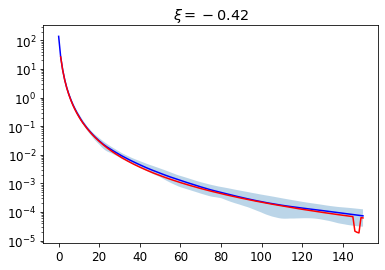
\includegraphics[width= 0.4 \textwidth]{new_imgs/stable xi.png}
    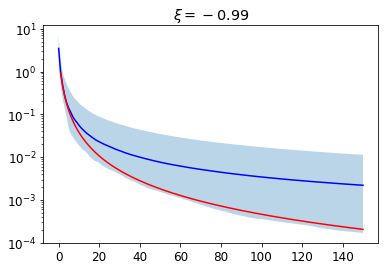
\includegraphics[width= 0.4 \textwidth]{new_imgs/unstable xi.png}
    \caption{Empirical vs Theoretical function-value performance for $\text{GCM}(\alpha^\star,\beta^\star)$ . Red lines are given by numerical integration, shades are minimum and maximum values under 10 runs}
    \label{fig:my_label}
\end{figure}

\begin{figure}[H]
    \centering
    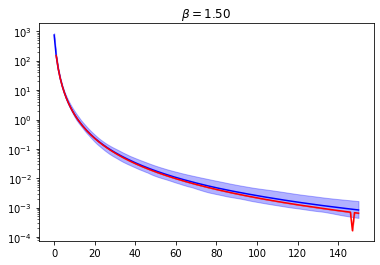
\includegraphics[width= 0.4 \textwidth]{new_imgs/stable beta.png}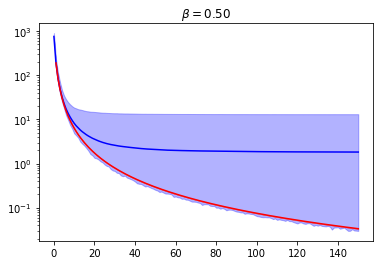
\includegraphics[width= 0.4 \textwidth]{new_imgs/unstable beta.png}
    \caption{Empirical vs Theoretical function-value performance under Marchenko Pastur distribution. Red lines are given by numerical integration,shades are minimum and maximum values under 10 runs}
    \label{fig:my_label}
\end{figure}
We note that in the regimes where the empirical average performance doesn't match the theoretical one, we can still find samples of problems who do match. This and the much larger variance on the function-value, this discrepancy is due to numerical unstability in these regimes.
\end{document}